\documentclass[Lau, oneside, noexaminfo]{sapthesis}

\usepackage[italian]{babel} 
\usepackage[utf8]{inputenx}
\usepackage{indentfirst}
\usepackage{microtype}
\usepackage{amsmath}

\usepackage{calligra}
\usepackage[T1]{fontenc}
\usepackage{amsfonts}
\usepackage{subfig}
\usepackage{multirow}
\usepackage{pgfplots}
\usepackage{cite}

%\usepackage[none]{hyphenat}

%\usepackage{chemformula}
%\usepackage{setspace}
%\usepackage{yfonts,color}
%\usepackage{siunitx}
%\usepackage{comment}
%\usepackage{multirow}
%\usepackage{varioref}
%\usepackage[bottom]{footmisc}
%\usepackage{wrapfig}
\usepackage{float}
%\usepackage{type1cm}
\usepackage{lettrine}
\linespread{0.9}
%\usepackage{chngcntr}
\usepackage[nottoc, notlof, notlot]{tocbibind}
%\onehalfspacing
%\counterwithout{footnote}{chapter}
\usepackage{hyperref}
\hypersetup{
			%hyperfootnotes=true,			
			%bookmarks=true,			
			colorlinks=true,
			linkcolor=red,
                        linktoc=page,
			anchorcolor=black,
			citecolor=red,
			urlcolor=blue,
			pdftitle={A sample Bachelor's thesis for Sapienza Università di Roma},
			pdfauthor={FirstName LastName},
			pdfkeywords={thesis, sapienza, roma, university}
			}

\title{Reti neurali convoluzionali per il riconoscimento di immagini mediche: analisi di attacchi di tipo adversarial e delle tecniche di difesa}
\author{Chiara Ballanti}
\IDnumber{1844613}
\course[]{Informatica}
\courseorganizer{Facoltà di Ingegneria dell’informazione, informatica e statistica}
\submitdate{2020/2021}
\copyyear{2021}
\advisor{Prof. Emiliano Casalicchio}                                                                                            
\authoremail{ballanti.1844613@studenti.uniroma1.it}

%we refer to http://ctan.mirrorcatalogs.com/macros/latex/contrib/sapthesis/sapthesis-doc.pdf for an exhaustive description of the sapthesis documentclass.


\begin{document}

\frontmatter
\maketitle

    \begin{abstract}
    Negli ultimi anni le Deep Neural Networks (DNNs) sono diventate sempre più popolari in numerose discipline come, ad esempio, Computer Vision (CV) e Natural Language Processing (NLP).
    
    L'evoluzione dei sistemi hardware ha contribuito allo sviluppo di potenti modelli di Deep Learning (DL) in grado di affrontare problemi complessi e impegnativi.
    
    Una delle sfide più importanti nel campo della CV è l'analisi delle immagini mediche - come la risonanza magnetica (MRI), i raggi X, la tomografia computerizzata (CT), la fondoscopia - utilizzando le Convolutional Neural Networks (CNNs) per la diagnosi di patologie o il rilevamento di disturbi specifici.
    
    Il corretto funzionamento di questi modelli può migliorare significativamente l'efficienza dei sistemi sanitari.
    
    Tuttavia, studi recenti hanno dimostrato che i modelli CNN sono vulnerabili agli adversarial attacks e che possono essere facilmente ingannati attraverso perturbazioni delle immagini impercettibili all'occhio umano.
    
    L'oggetto di questa tesi è lo studio di alcune tecniche esistenti di adversarial attacks, il loro rilevamento e le tecniche di difesa per le immagini mediche.
    \end{abstract}

\tableofcontents

\mainmatter

\chapter{Introduzione}
\label{chap:1}

Le tecniche di Machine Learning (ML), specialmente i recenti modelli di Deep Learning (DL), stanno progredendo rapidamente e sono sempre più impiegate in vari ambiti.

Le Convolutional Neural Networks (CNNs) sono tra i più importanti tipi di modelli DL utilizzati per l'elaborazione e l'analisi delle immagini, poiché sono molto efficaci nell'estrazione di caratteristiche fondamentali dall'immagine, ovvero parti o schemi di un oggetto che aiutano ad identificarlo.

Alcune delle discipline più rappresentative che usano il DL per compiti di Computer Vision (CV) sono la robotica, i veicoli autonomi, la biometria, il riconoscimento dei volti e la classificazione delle immagini.

In seguito al suo successo, il DL è diventato un utile strumento di supporto per l'analisi di immagini mediche, poiché permette ai medici di svolgere i loro compiti in modo più efficiente e in minor tempo.
Nell'analisi delle immagini mediche, gli algoritmi di DL possono analizzare ed elaborare la risonanza magnetica, la TAC, i raggi X e le immagini della pelle per la diagnosi del cancro, il rilevamento della retinopatia, la classificazione delle malattie polmonari, i tumori del cervello, ecc.
Anche se gli algoritmi di DL riescono a raggiungere performance molto alte, a volte anche superiori a quelle umane, alcuni studi hanno dimostrato che possono essere vulnerabili agli adversarial attacks. 

Gli adversarial attacks vengono applicati introducendo intenzionalmente delle piccole perturbazioni nei dati di input dell'algoritmo di DL. 
In %[bibl: https://arxiv.org/pdf/1312.6199.pdf] 
\cite{szegedy2013intriguing} gli autori hanno dimostrato che una piccolissima perturbazione su un'immagine può portare il modello di DL a conclusioni errate. 
La perturbazione aggiunta ad un'immagine pulita può essere casuale oppure calcolata al fine di massimizzare l'errore di predizione. 
Questi tipi di attacchi sono particolarmente efficaci perché le perturbazioni sono impercettibili all'occhio umano, rendendo così, per una persona, le immagini perturbate indistinguibili da quelle pulite.

Inoltre, esiste un fenomeno denominato \textbf{adversarial transferability} %[bibl: https://arxiv.org/pdf/1605.07277.pdf] 
\cite{papernot2016transferability} che permette a degli adversarial examples, appositamente creati per un modello, di poterne ingannare efficacemente anche altri.

Gli adversarial attacks hanno sollevato, nella comunità di ricerca, preoccupazioni sulla sicurezza e affidabilità delle DNN e sull'opportunità di delegare diagnosi mediche a questi modelli, che possono essere facilmente ingannati. 
La consapevolezza di queste problematiche ha indotto la comunità di ricerca a cercare delle soluzioni per rendere questi modelli più robusti e sicuri.

\bigskip
Il \hyperref[chap:2]{Capitolo~\ref*{chap:2}} presenta l'analisi della letteratura effettuata nell'ambito di questo lavoro di tesi.

\bigskip
Nel \hyperref[chap:3]{Capitolo~\ref*{chap:3}} viene spiegato il problema nello specifico e le motivazioni per cui questi attacchi vengono effettuati anche in ambito medico. In particolare, vengono illustrati in dettaglio gli attacchi presi in esame durante il lavoro di tesi e alcune delle tecniche di difesa applicate al fine di mitigarli. 

\bigskip
Nel \hyperref[chap:4]{Capitolo~\ref*{chap:4}} vengono descritti gli esperimenti sugli attacchi: i datasets, le architetture dei modelli CNN e gli esiti prodotti dagli attacchi.

\bigskip
Nel \hyperref[chap:5]{Capitolo~\ref*{chap:5}} vengono esposti i risultati degli esperimenti sulla difesa dei modelli scelti.

\bigskip
Per visionare il codice sorgente implementato durante il lavoro di tesi e tutti gli esperimenti effettuati si faccia riferimento a GitHub \cite{MyGitHub}.

\chapter{Analisi della letteratura}
\label{chap:2}

    \paragraph{Dizionario dei termini}
        In questo paragrafo, si illustrano i termini tecnici comunemente utilizzati nella letteratura per descrivere gli adversarial attacks applicati al deep learning in Computer Vision:
            \begin{itemize}
                \item \textbf{Adversarial example/image} (Immagine/esempio avversario): è una versione modificata di un'immagine pulita che viene intenzionalmente perturbata (ad esempio aggiungendo del rumore) per confondere/ingannare una tecnica di apprendimento automatico, come le DNN.
                \item \textbf{Adversarial perturbation/noise} (Perturbazione avversaria/rumore): è il rumore che viene aggiunto ad un'immagine pulita per renderla un adversarial example.
                \item \textbf{Adversary} (Avversario): si riferisce più comunemente all'agente che crea un esempio avversario.
                \item \textbf{Modello/classificatore/algoritmo di classificazione}: è l'algoritmo che prende in input un'immagine e la riconosce restituendo in output la sua etichetta/classe. È la tecnica di apprendimento automatico che analizza l'immagine e la classifica.
            \end{itemize}

\section{Adversarial Attacks}
Nella figura \ref{Panda}, è possibile vedere come l'immagine iniziale venga classificata correttamente come un panda mentre, con l'aggiunta di un rumore molto piccolo, il modello classifichi con sicurezza il panda come un gibbone.
    \begin{figure}[!h]
        \centering
        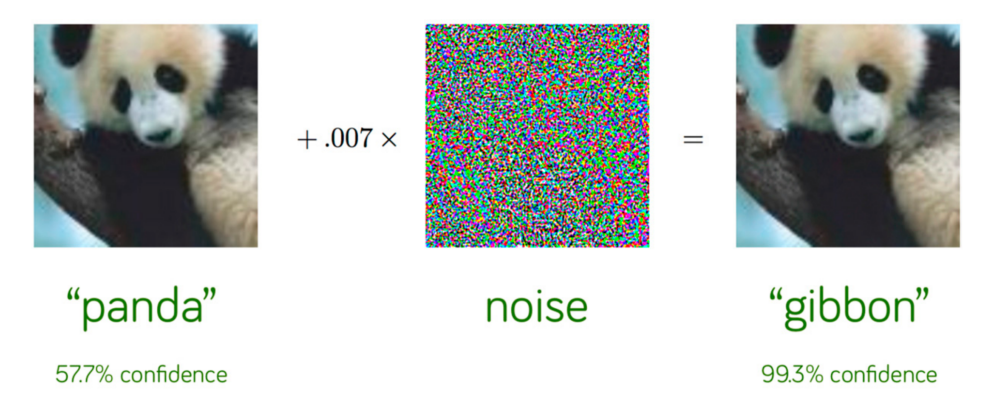
\includegraphics[width=0.7\textwidth]{Images/Panda.png}
        \caption{Previsione del modello prima e dopo l'attacco.}
        \label{Panda}
    \end{figure}

Le prime spiegazioni sugli adversarial attacks riguardavano la non linearità e l'overfitting mentre, successivamente, Goodfellow %[https://arxiv.org/pdf/1412.6572.pdf] 
\cite{goodfellow2014explaining} ha dimostrato che %la ragione di tale vulnerabilità è proprio la linearità dei modelli.
anche i modelli lineari erano altamente vulnerabili.
Anche altri studi hanno cercato di spiegare questo fenomeno. Schmid %[https://arxiv.org/pdf/1804.11285.pdf] 
\cite{schmidt2018adversarially} sostiene che il successo degli adversarial attacks sia dovuto alla carenza di dati reali e alla loro distribuzione non omogenea. Ilyas %[https://arxiv.org/pdf/1905.02175.pdf] 
\cite{ilyas2019adversarial} afferma che questi attacchi sono efficaci a causa delle capacità di generalizzazione dei modelli su un dataset specifico: il modello estrae così features altamente prevedibili ma non robuste.\\

Finora, la maggior parte degli studi esistenti sono stati effettuati su immagini naturali. Le immagini naturali hanno numerose differenze rispetto alle immagini mediche e questo è un motivo fondamentale per studiare come gli adversarial attacks influenzano le immagini mediche.

Prima di tutto, si ha un'insufficienza di grandi datasets di immagini mediche con etichette annesse a causa dell'elevato costo e del consumo di tempo che comporta la raccolta dei dati. Inoltre, la classe normale è spesso sovrarappresentata, portando quindi ad una convergenza lenta e al problema dell'overfitting.

Un'altra differenza tra questi due tipi di immagini è che i dati medici spesso contengono informazioni quantitative mentre le immagini naturali no. 

Inoltre, ci sono munerosi casi in cui le differenze tra le classi sono molto piccole.
Ad esempio, una radiografia con una polmonite allo stadio iniziale è abbastanza simile ad una radiografia normale. 

In aggiunta, le immagini naturali sono generate da telecamere RGB, mentre la maggior parte delle immagini mediche non lo sono. 

Tuttavia, numerosi studi hanno dimostrato che anche le immagini mediche possono essere influenzate da adversarial attacks. %[https://www.medrxiv.org/content/10.1101/2021.01.17.21249704v1.full, https://www.ncbi.nlm.nih.gov/pmc/articles/PMC7738012/, https://www.sciencedirect.com/science/article/pii/S1361841521001870?via%3Dihub#sec0010].
Ad esempio le immagini oncologiche \cite{joel2021adversarial}, le immagini dermatologiche \cite{allyn2020adversarial} e le fondoscopie \cite{bortsova2021adversarial}.

Ma è stato provato %[https://arxiv.org/pdf/1907.10456.pdf] 
\cite{ma2021understanding} che i modelli DL medici sono più vulnerabili dei modelli di immagini naturali per due motivi: 
    \begin{enumerate}
        \item la caratteristica texture biologica delle immagini mediche ha molte aree che possono essere facilmente ingannate;
        \item i moderni modelli DL sono costituiti da molti livelli in quanto sono stati progettati per l'elaborazione delle immagini naturali. Introducono quindi un elevato numero di parametri che, nel caso dell'analisi delle immagini mediche, può portare ad una iper-parametrizzazione ed aumentare la vulnerabilità del modello.
    \end{enumerate}

Nonostante ciò, gli attacchi nelle immagini mediche sono rilevati più facilmente che in un'immagine naturale, poiché le caratteristiche avversarie sono linearmente separate dalle caratteristiche normali, mentre nelle immagini naturali gli adversarial examples sono simili ai normali.

\newpage

\section{Mitigation di Adversarial Attacks}
Al fine di ridurre la vulnerabilità dei modelli DL, nel corso degli ultimi anni sono state studiate numerose tecniche di difesa per mitigare gli adversarial attacks.

\paragraph{Input Denoising}
Poiché un adversarial attack consiste nell'aggiungere ai dati un rumore impercettibile all'occhio umano, allora una soluzione di difesa naturale potrebbe essere quella di provare ad eliminare la perturbazione.

Formalmente, dati un'immagine pulita $x$, il rispettivo adversarial example $x_{adv}$ e un modello di classificazione $f$, si cerca di progettare una mappatura $f_m$ tale che $f(f_m(x_{adv})) = f(x)$.

Recentemente sono state sviluppate delle difese che ricorrono a schemi di randomizzazione per eliminare le perturbazioni avversarie. 

L'intuizione dietro questo tipo di difesa è che le DNN sono da sempre robuste alle perturbazioni casuali. Una difesa basata sulla randomizzazione cerca di randomizzare i rumori avversari in rumori casuali, che non sono una preoccupazione per la maggior parte delle DNN. 
\\

Tra queste tecniche troviamo il Feature Squeezing \cite{xu2017feature}, che consiste nell'utilizzo di due metodi di squeezing, riduzione dei bit e sfocatura dell'immagine. 
Il rilevamento dell'adversarial example è realizzato confrontando le previsioni del modello sulle immagini originali e quelle prodotte dagli squeezing. Se i due input passati al modello producono output sensibilmente diversi, è probabile che l'input originale sia un adversarial example. Nonostante il Feature Squeezing risulti una tecnica di difesa molto efficace contro attacchi potenti come C\&W (Carlini \& Wagner), è stato dimostrato \cite{he2017adversarial, sharma2018bypassing} che è ancora troppo vulnerabile.
\\

Un altro modo per riportare le immagini al loro stato iniziale è l'impiego delle Generative Adversarial Networks (GANs).
Una GAN è un potente strumento in grado di apprendere un modello generativo per le distribuzioni di dati. Per questo molti studi le sfruttano per apprendere distribuzioni di dati puliti al fine di generare, per ogni adversarial example, la rispettiva controparte pulita. 

Due esempi sono Defense-GAN \cite{samangouei2018defense} e Adversarial perturbation elimination GAN (APE-GAN) \cite{shen2017ape}. 

Defense-GAN traina un generatore per modellare la distribuzione delle immagini pulite. Durante la fase di testing, Defense-GAN elimina la perturbazione avversaria cercando un'immagine vicina all'adversarial example in input nella distribuzione appresa. Restituisce quindi un'immagine pulita che darà in input al classificatore.
Questa strategia può essere utilizzata per difendersi da vari adversarial attacks, ma non tutti. Attualmente, lo schema di attacco più efficace contro Defense-GAN è basato su una tecnica chiamata \textit{Backward
Pass Differentiable Approximation} \cite{athalye2018obfuscated}, ed è in grado di ridurre la sua precisione fino al 55\%. 

APE-GAN traina direttamente un generatore per pulire un adversarial example, preso in input, e genera una controparte pulita. Anche se APE-GAN raggiunge buoni risultati \cite{shen2017ape}, l'attacco white-box proposto da Carlini e Wagner \cite{carlini2017magnet} può facilmente sconfiggerla. 

\paragraph{Model Robustification}
Un'altra strategia ampiamente adottata consiste nel raffinare il modello per prepararsi ad affrontare una potenziale minaccia.
Il perfezionamento del modello potrebbe essere ottenuto in due modi: cambiando l'obiettivo della fase di training o modificando la struttura del modello.
\\

Nel primo caso, l'idea di base è quella di considerare la minaccia degli adversarial attacks e rendere il modello più robusto durante la fase di training. 

Una di queste tecniche è l'Adversarial Training \cite{goodfellow2014explaining}, durante il quale il modello viene addestrato con immagini pulite e perturbate, entrambe etichettate correttamente.
\\

Esempi di modifica del modello includono la Model Distillation \cite{papernot2015distillation}, che utilizza le conoscenze del modello per migliorare la propria robustezza. Le conoscenze vengono estratte sotto forma di vettori di classi di probabilità dei dati di training e vengono date in input al modello originale per trainarlo nuovamente.
\\

Formalmente, dati un'immagine pulita $x$, il rispettivo adversarial example $x_{adv}$, la rispettiva classe $y$ e un modello di classificazione $f$, si cerca di progettare un modello robusto $f'$, basato su $f$, tale che $f'(x_{adv}) = f'(x) = y$.


\paragraph{Adversarial Detection}
Nelle due strategie precedenti, data un'istanza $x$, si cerca di predire la sua vera classe. L'Adversarial Detection, invece, mira a stabilire se un'istanza data è un adversarial examples.

Formalmente, data un'immagine $x'$, si cerca di progettare un modello $f_d$ tale che $f_d(x') = 1$ se e solo se $x'$ è un adversarial examples, altrimenti $f_d(x') = 0$.
\\

Una tecnica di difesa di questo tipo è MagNet \cite{meng2017magnet}, che include un detector ed un reformer, ed utilizza un autoencoder per imparare la distribuzione dei campioni puliti. Il detector distingue i campioni puliti e quelli avversari in base alle relazioni tra questi campioni e la distribuzione appresa. Il reformer è progettato per rettificare gli adversarial examples in campioni puliti. MagNet risulta efficace contro una varietà di adversarial attacks sotto impostazioni gray-box e black-box, come FGSM, BIM, e C\&W. Tuttavia, Carlini e Wagner \cite{carlini2017magnet} dimostrano che MagNet è vulnerabile agli adversarial examples trasferibili generati da un attacco.

\chapter{Descrizione del problema}
\label{chap:3}
    
    \paragraph{Medical Image Analysis}
    L'analisi delle immagini mediche ha lo scopo di esaminare il corpo umano per motivi medici come la diagnosi, i trattamenti e il monitoraggio della salute. Con il passare degli anni le DNN si sono rivelate la scelta migliore per trattare dati complessi e ad alta dimensione come le immagini mediche. L'uso della Computer Vision (CV) in medicina è significativo perché offre alti tassi di successo nella diagnosi precoce, fondamentale per ridurre i tassi di mortalità. Inoltre, l'analisi delle immagini mediche diminuisce gli errori di singoli operatori medici. Uno studio %[bibl: https://pubmed.ncbi.nlm.nih.gov/27143499/] 
    \cite{makary2016medical} ha dimostrato che gli errori medici sono la terza causa di morte negli Stati Uniti. Ciò significa che l'impiego delle DNN in ambito medico può aumentare le aspettative di vita umana.
    
    Sono numerosi gli ambiti dell'analisi delle immagini mediche di cui si occupa il DL e i più importanti sono: classificazione o diagnosi (classification), rilevamento (detection) e segmentazione (segmentation).
    
    Il lavoro di tesi si concentra sulla classificazione.
    
    \paragraph{Classificazione}
    Una delle principali aree di applicazione del DL nell'analisi delle immagini mediche è la classificazione, detta anche \textit{computer-aided-diagnosis} (CAD), ovvero la diagnosi assistita dal computer in cui le immagini sono input e i modelli DL classificano le immagini in una o più classi.
    
    Risale al 1995 uno dei primi studi %[bibl: https://www.researchgate.net/profile/Seong-Mun/publication/3220638_Artificial_Convolution_Neural_Network_Techniques_and_Applications_for_Lung_Nodule_Detection/links/59cd2a09a6fdcc0333ebcd74/Artificial-Convolution-Neural-Network-Techniques-and-Applications-for-Lung-Nodule-Detection.pdf], 
    \cite{lo1995artificial}, in cui è stata usata una CNN con due \textit{hidden layers} per diagnosticare se un'immagine a raggi X raffigurasse dei noduli polmonari oppure no.
    In un altro studio %[bibl: https://arxiv.org/pdf/1711.05225.pdf] 
    \cite{rajpurkar2017chexnet} è stato sviluppato il modello CheXNet, modificando il modello preesistente DenseNet121, per classificare un dataset di radiografie al torace in 14 disturbi polmonari. 
    La retinopatia diabetica (DR) è un altro metodo di diagnosi ben noto per i modelli DL. In tale ambito, Korolev %[bibl: https://arxiv.org/pdf/1701.06643.pdf] 
    \cite{korolev2017residual} ha ideato un nuovo modello, basato sulle architetture VGGNet e ResNet, per la diagnosi di Alzheimer.
    
    \paragraph{Adversarial attacks in ambito medico}
    Una decisione sbagliata in medicina può avere un costo molto elevato in termini di vite umane.
    Anche se gli adversarial attacks sembrano improbabili nell'analisi delle immagini mediche, ci sono alcune serie considerazioni che dovrebbero essere prese in esame:
        \begin{itemize}
            \item una decisione sbagliata può avere ripercussioni pericolose sulla vita di un paziente e può comportare costi aggiuntivi elevati e/o l'inutile impiego di risorse sanitarie.
            \item un paziente può perturbare il referto di un esame con l'obiettivo di ricevere un risarcimento assicurativo.
            \item un medico malintenzionato può sfruttare l'attacco a proprio vantaggio per scopi di lucro. Può, infatti, manipolare i referti degli esami per poter intervenire laddove non ce ne sia bisogno. Ad esempio, potrebbe effettuare un intervento chirurgico non necessario e/o potrebbe indurre un paziente ad assumere un farmaco di cui non ha necessità.
        \end{itemize}
        
    
    \newpage
    
\section{Tecniche di Intelligenza Artificiale }
    
    \subsection{Artificial Neural Networks (ANN)}
        
        \paragraph{Cos'è una rete neurale artificiale?}
        Ispirata al cervello umano con le sue miliardi di connessioni, una Artificial Neural Network (o rete neurale artificiale) si compone di numerosi strati di unità interconnesse chiamate neurons (o neuroni). I neuroni sono raggruppati in layers (o strati). A seconda dei segnali che riceve in input, un neurone può essere attivato, producendo a sua volta un altro segnale da inviare ad un altro neurone. 
            \begin{figure}[!h]
                \centering
                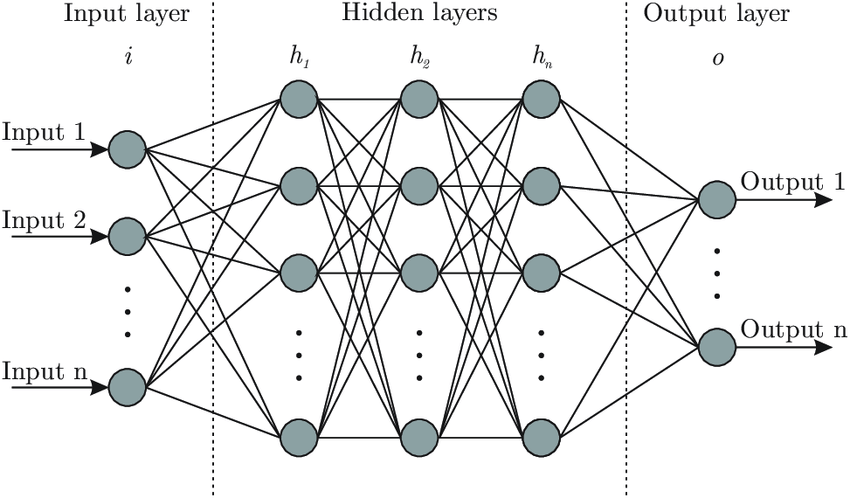
\includegraphics[width=0.8\textwidth]{Images/NN/ANN.png}
                \caption{Architettura di una rete neurale artificiale}
                \label{ANN architecture}
            \end{figure}
        
        Come mostrato nella figura \ref{ANN architecture}, l'insieme dei segnali che la ANN riceve in input si propaga attraverso gli strati intermedi, chiamati hidden layers (o strati nascosti) ed infine allo strato di output.

        \paragraph{Neurone artificiale}
        I neuroni sono gli elementi costitutivi delle reti neurali.
            \begin{figure}
                \centering
                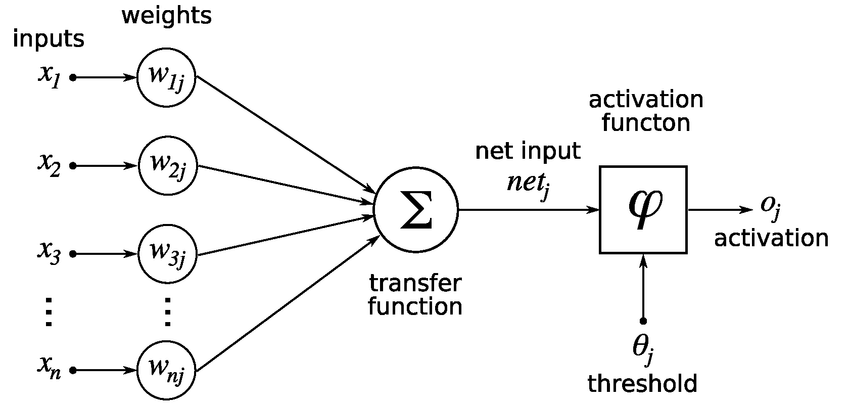
\includegraphics[width=0.7\textwidth]{Images/NN/Neuron.png}
                \caption{Struttura di un neurone}
                \label{Neuron}
            \end{figure}
        La figura \ref{Neuron} mostra una delle strutture base di un neurone. Un insieme di valori di input sono pesati e sommati. Questo risultato è usato come input per una activation function (o funzione di attivazione) che determina quanto il neurone sarà attivato dal segnale di input ricevuto.
        
        Per questo motivo, l'analogia con il cervello umano è forte, un neurone biologico è attivato da qualche segnale di input e propaga il suo output ad altri. 
        
        Le variabili della figura \ref{Neuron} sono di seguito riportate:
            \begin{itemize}
                \item $x_i$: è uno dei valori in input
                \item $w_i$: è uno dei pesi
                \item $\theta$: è la soglia di attivazione
            \end{itemize}
        
        \paragraph{Algoritmo di retropropagazione}
        L'algoritmo di back propagation (o retropropagazione) è un algoritmo di apprendimento delle reti neurali. L'algoritmo confronta il valore in output della ANN con il valore desiderato (obiettivo). Sulla base della differenza così calcolata (errore), l'algoritmo modifica i pesi sinaptici della rete neurale, facendo convergere progressivamente il set dei valori di output verso quelli desiderati.
        
    \newpage    
    \subsection{Convolutional Neural Networks (CNN)}
        
        \paragraph{Cos'è una rete neurale convoluzionale?}
        Una Convolutional Neural Network (o rete neurale convoluzionale) è una classe di reti neurali specializzata nell'elaborazione di dati che hanno una topologia a griglia, come un'immagine.\\
            \begin{figure}[!h]
                \centering
                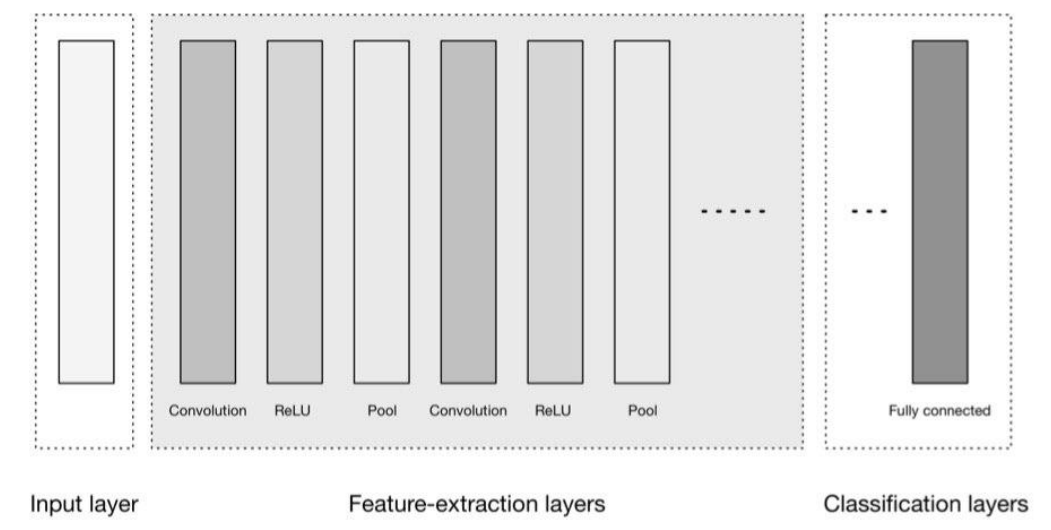
\includegraphics[width=0.8\textwidth]{Images/NN/CNN.png}
                \caption{Panoramica ad alto livello della struttura di una CNN}
                \label{CNN architecture}
            \end{figure}
        
        La figura \ref{CNN architecture} mostra una panoramica ad alto livello dell'organizzazione di una CNN. Oltre allo strato di input, gli strati intermedi realizzano l'estrazione delle caratteristiche mentre la parte finale completamente connessa esegue la classificazione.
        
        Nelle architetture CNN di base, l'estrazione delle caratteristiche viene eseguita con uno schema ripetuto. Prima, l'input attraversa uno strato di convoluzione, poi viene applicata una funzione di attivazione (generalmente la ReLU) e, infine, passa per uno strato di pooling, che riduce la dimensione delle informazioni.
        
        \paragraph{Convolution Layer}
        Il Convolutional layer (o strato di convoluzione) è il blocco fondamentale della CNN. Il suo ruolo è quello di trovare la congiunzione locale tra le caratteristiche degli strati precedenti.
        
        I weights (o pesi) in una rete neurale convoluzionale sono raggruppati in matrici chiamate kernels (o filtri).
            \begin{figure}[!h]
                \centering
                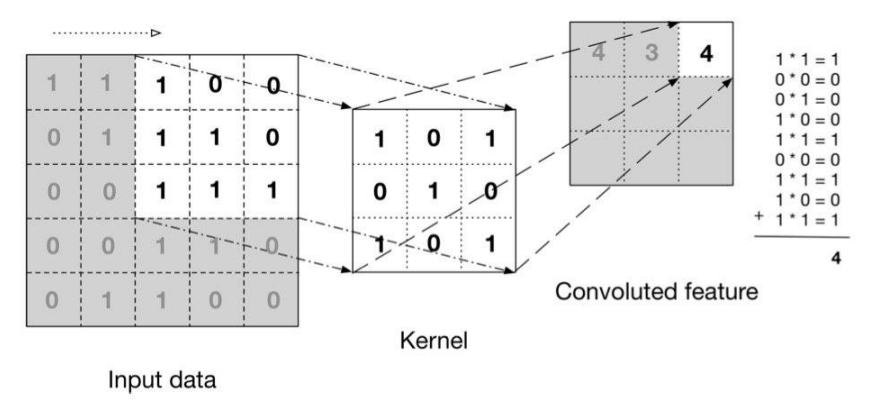
\includegraphics[width=0.7\textwidth]{Images/NN/Convolutional Layer.png}
                \caption{Operazione di convoluzione}
                \label{Convolution}
            \end{figure}
        
        \newpage
        Come mostrato in figura \ref{Convolution} l'operazione di convoluzione viene applicata moltiplicando un kernel per un'area dell'immagine di input (ogni valore viene moltiplicato per il peso corrispondente, quindi il risultato è la somma di tutte le moltiplicazioni). Il risultato viene memorizzato nella matrice di output chiamata mappa delle caratteristiche o mappa di attivazione. Ci sono molti di questi kernels. Una volta che l'input è stato completamente elaborato, la rete utilizza il kernel successivo. 
        
        È importante notare che la profondità della mappa di attivazione non è legata all'input o alla profondità del kernel, ma è uguale al numero di kernel applicati all'immagine di input.\\
        
        Alcune definizioni per questo strato:
            \begin{itemize}
                \item N: larghezza/altezza dell'input, nel caso semplificato di un'immagine di input quadrata.
                \item P: la quantità di padding usata nell'input. Il padding è utile per ottenere una dimensione desiderata nella mappa di attivazione, per esempio, per mantenere le stesse dimensioni dell'input.
                \item S: lo stride. Esprime di quanto viene spostato un kernel durante la convoluzione.
                \item F: la dimensione del kernel.
            \end{itemize}
        
        La dimensione della mappa delle caratteristiche di output è: 
            \begin{equation}
                \left\lfloor\frac{N + 2P - F}{S}\right\rfloor + 1
            \end{equation}

        \paragraph{Pooling Layer}
        Il Pooling Layer (o strato di pooling) raggruppa caratteristiche semanticamente simili trovate nella precedente mappa di attivazione e aiuta a controllare l'overfitting.
        
        Gli strati di pooling più comuni sono il Max-pooling layer, che estrae il valore massimo, e il Average-pooling layer, che calcola la media dei valori.
            \begin{figure}[!h]
                \centering
                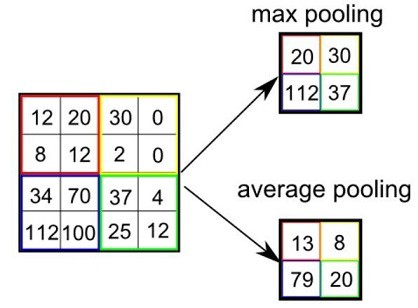
\includegraphics[width=0.3\textwidth]{Images/NN/Pooling Layer.jpeg}
                \caption{Esempio di Max-pooling e Average-pooling.
                I diversi colori evidenziano diverse aree dell'input allo strato di polling.}
                \label{Pooling}
            \end{figure}
        
        \paragraph{Fully Connected Layer}
        Il Fully Connected Layer (o strato completamente connesso) prende l'output dello strato di convoluzione/pooling, lo appiattisce e predice la migliore etichetta per descrivere l'immagine. Come in una normale rete neurale feed-forward, gli ingressi allo strato completamente connesso sono moltiplicati per i pesi e sommati insieme. Poi viene utilizzata una funzione di attivazione  per produrre l'output. I risultati sono propagati allo strato successivo completamente connesso. L'ultimo ha un neurone per ogni etichetta di classe e produce la distribuzione di probabilità.

        \paragraph{Non-Linearity Layers}
        Poiché la convoluzione è un'operazione lineare e le immagini sono tutt'altro che lineari, i Non-Linearity Layers (o strati di non linearità) sono spesso posti direttamente dopo lo strato di convoluzione per introdurre la non linearità nella mappa di attivazione.\\
        
        Ci sono diversi tipi di operazioni non lineari, le più popolari sono:
            \begin{itemize}
                \item \textbf{Sigmoid}: funzione che prende un numero reale e lo standardizza in un intervallo tra 0 e 1.\\
                    \begin{center}
                        \resizebox{8cm}{!} {
                            \begin{tikzpicture}
                                \begin{axis}[
                                    axis lines = left,
                                    xlabel = \(x\),
                                    ylabel = {\(f(x)\)},
                                    legend pos=outer north east,
                                    legend style={nodes={scale=1.5, transform shape}}
                                ]
                                \addlegendimage{empty legend}
                                \addplot [
                                    domain=-10:10, 
                                    samples=100, 
                                    color=red,
                                    ultra thick,
                                ]
                                {1/(1+e^(-x))};
                                
                                \addlegendentry{\hspace{-.3cm}\textbf{Sigmoide}}
                                \addlegendentry{$\frac{1}{1+e^{-x}}$}
                                \end{axis}
                            \end{tikzpicture}
                        }
                    \end{center}
                \item \textbf{Tanh}: funzione che prende un numero reale e lo standardizza in un intervallo tra -1 e 1.\\
                    \begin{center}    
                        \resizebox{8cm}{!} {
                            \begin{tikzpicture}
                                \begin{axis}[
                                    axis lines = left,
                                    xlabel = \(x\),
                                    ylabel = {\(f(x)\)},
                                    legend pos=outer north east,
                                    legend style={nodes={scale=1.5, transform shape}}
                                ]
                                \addlegendimage{empty legend}
                                \addplot [
                                    domain=-10:10, 
                                    samples=100, 
                                    color=red,
                                    ultra thick,
                                ]
                                {tanh(x)};
                                
                                \addlegendentry{\hspace{-.3cm}\textbf{Tanh}}
                                \addlegendentry{$\tanh{x}$} 
                                \end{axis}
                            \end{tikzpicture}
                    }
                    \end{center}
                \item \textbf{Rectified Linear Unit (ReLU)} 
                    \begin{center}    
                        \resizebox{8cm}{!} {
                            \begin{tikzpicture}
                                \begin{axis}[
                                    axis lines = left,
                                    xlabel = \(x\),
                                    ylabel = {\(f(x)\)},
                                    legend pos=outer north east,
                                    legend style={nodes={scale=1.5, transform shape}} 
                                ]
                                \addlegendimage{empty legend}
                                \addplot [
                                    domain=-10:10, 
                                    samples=100, 
                                    color=red,
                                    ultra thick,
                                ]
                                {max(0, x)};
                                
                                \addlegendentry{\hspace{-.3cm}\textbf{ReLU}}
                                \addlegendentry{$\max(0, x)$} 
                                \end{axis}
                            \end{tikzpicture}
                        }
                    \end{center}
            \end{itemize}
\newpage  
        \paragraph{Classification problem}
        Le CNN sono ritenute le reti neurali più efficienti quando si tratta di risolvere i problemi di classificazione.
        
        Per un classification problem (o problema di classificatione) a $K$-classi ($K \geq 2$), dato un dataset $\{(x_i, y_i)\}_{i=1,...,N}$ dove $x_i \in \mathbb{R}^d$ è un'immagine pulita e $y_i \in \{1, ... , K\}$ è la sua classe, un classificatore DNN $h$ con parametri $\theta$ predice la classe di un input $x_i$:
            \begin{equation}
                h(x_i) = \operatorname*{arg\,max}_{k = 1, ..., K}p_k(x_i, \theta)
            \end{equation}
        dove
            \begin{equation}
                p_k(x_i, \theta) = \frac{\text{exp}(z_k(x_i, \theta))}{\sum_{k'=1}^{K}\text{exp}(z_{k'}(x_i, \theta))}
            \end{equation}
        dove $z_k(x_i, \theta)$ è il logits output della rete rispetto alla classe $k$, e $p_k(x_i, \theta)$ è la probabilità (softmax su logits) che $x_i$ appartenga alla classe $k$. I parametri $\theta$ del modello sono aggiornati usando la back-propagation per minimizzare la classification loss.
\newpage
\section{Tecniche di Adversarial Attacks}
\label{Tecniche di Adversarial Attacks}

    \paragraph{Cos'è un adversarial attack}
    Dato un modello pre-trainato $h$ e un'immagine pulita $x$ associata ad un'etichetta di classe $y$, un metodo di attacco consiste nel massimizzare l'errore di classificazione del modello DNN, mantenendo $x_{adv}$ all'interno di una piccola \textit{$\epsilon$-ball} centrata sul campione originale $x$ $(||x_{adv}-x||_p \leq \epsilon)$, dove $||\cdot||_p$ è la $L_p$-\textit{norm}, sapendo che $L_\infty$ è la norma più utilizzata a causa della sua consistenza rispetto alla percezione umana.\\
    \newline
    Un adversarial attack può essere \textit{targeted} o \textit{untargeted}:
        \begin{itemize}
            \item Un \textbf{targeted attack} consiste nel trovare un adversarial example $x_{adv}$ che venga classificato della DNN in una classe specifica $h(x_{adv} \neq y_{target})$ diversa dalla classe reale di $x$ $(y_{target} \neq y)$
            \item Un \textbf{untargeted attack} consiste nel trovare un adversarial example $x_{adv}$ che venga classificato in modo errato della DNN in una classe arbitraria $h(x_{adv} \neq y)$
        \end{itemize}
    Un adversarial attack può essere \textit{white-box} o \textit{black-box}:
        \begin{itemize}
            \item Un \textbf{white-box attack} presume la conoscenza completa del modello attaccato, compresi i valori dei parametri, l'architettura, il metodo di addestramento e, più raramente, anche i dati utilizzati durante quest'ultimo.
            \item Un \textbf{black-box attack} alimenta un modello mirato con adversarial examples (durante i test) generati senza avere alcuna conoscenza di quel modello. 
            \item In alcuni casi, si presume che l'avversario abbia una conoscenza limitata del modello (ad esempio la sua procedura di addestramento e/o la sua architettura), ma sicuramente non conosce il modello.In altri casi, l'utilizzo di qualsiasi informazione sul modello di destinazione è indicato come \textit{semi-black-box attack}.
        \end{itemize}
    Nel documento verranno analizzati untargeted e targeted attacks in ambiente white-box sotto il vincolo di perturbazione $L_\infty$.\\ 
    \newline
    Per gli \textit{white-box untargeted attacks}, gli adversarial examples vengono generati risolvendo il seguente problema di ottimizzazione vincolata:
        \begin{equation}
            x_{adv}=\operatorname*{arg\,max}_{||x'-x||_\infty \leq \epsilon}l(h(x'),y)
        \end{equation}
        dove $l(\cdot)$ è la classification loss, e $y$ è la classe reale.\\
    \newline
    Per gli \textit{white-box targeted attacks}, gli adversarial examples vengono generati risolvendo il seguente problema di ottimizzazione vincolata:
        \begin{equation}
            x_{adv}=\operatorname*{arg\,min}_{||x'-x||_\infty \leq \epsilon}l(h(x'),y_{target})
        \end{equation}
        dove $l(\cdot)$ è la classification loss, e $y$ è la classe target diversa da quella reale.
    \newpage

    \paragraph{Attacchi} Nella seguente tabella si riportano gli attacchi considerati durante il lavoro di tesi:
        \begin{table}[!h]
            \centering
            \begin{tabular}{|c|c|c|c|c|}
                \hline
                \rule[-3mm]{0mm}{8mm}
                \textbf{Attack}   &\textbf{Target}  & \textbf{Settings} & \textbf{Perturbation Norm} & \textbf{Learning}  \\ \hline \hline
                \rule[-3mm]{0mm}{8mm}
                FGSM     & Targeted             & White-Box       & $l_\infty$        & One-shot  \\ \hline
                \rule[-3mm]{0mm}{8mm}
                BIM      & Untargeted           & White-Box       & $l_\infty$        & Iterative \\ \hline
                \rule[-3mm]{0mm}{8mm}
                PGD      & Targeted             & White-Box       & $l_\infty$, $l_2$ & Iterative \\ \hline
                \rule[-3mm]{0mm}{8mm}
                DeepFool & Untargeted           & White-Box       & $l_\infty$, $l_2$ & Iterative \\ \hline
            \end{tabular}
            \caption{Riassunto degli attributi di diversi metodi di attacco.}
            \label{Tab Attacks}
        \end{table}
    
    \subsection{Fast Gradient Sign Method (FGSM)}
    \label{FGSM}
    Goodfellow \cite{goodfellow2014explaining} sviluppò un metodo per calcolare efficientemente un adversarial perturbation data un'immagine pulita, risolvendo la seguente equazione:
        \begin{equation}
            \eta = \epsilon\, \text{sign} (\nabla_x J(\theta, x, y))
        \end{equation}
        dove $x$ è l'immagine pulita in input, $y$ è la classe reale di $x$ e $\theta$ rappresenta i pesi del modello attaccato. Inoltre, $\epsilon$ è la magnitudine della perturbazione, un valore scalare arbitrariamente piccolo che limita la norma della perturbazione, $J(\theta, x, y)$ è la gradient loss, sign$(\cdot)$ è la sign function e $\nabla_x(\cdot)$ è il gradiente rispetto ad $x$.\\
    \newline
    L'adversarial example è calcolato come segue:
        \begin{equation}
            \begin{split}
                x_{adv} &= x + \eta \\
                        &= x + \epsilon\, \text{sign} (\nabla_x J(\theta, x, y))
            \end{split}
        \end{equation}
    Il Fast Gradient Sign Method è uno dei primi attacchi proposti per la generazione di adversarial examples.
    \newpage
    \subsection{Basic Iterative Method (BIM)}
    \label{BIM}
    Un metodo \textit{one-step} perturba le immagini facendo un unico grande passo nella direzione che aumenta la \textit{loss} del classificatore. Un'estensione intuitiva di questa idea consiste nel fare, iterativamente, più piccoli passi aggiustando la direzione dopo ogni passo.
    
    Il Basic Iterative Method (BIM) \cite{kurakin2016adversarial} è un'estensione dell'attacco FGSM e consiste nel ripetere quest'ultimo più volte usando un passo di lunghezza ridotta.
    
    Invece di applicare un adversarial noise $\eta$ una singola volta con un parametro $\epsilon$, lo si applica più volte, iterativamente, con uno step-size $\alpha$ molto piccolo.\\
    
    L’adversarial example è calcolato attraverso la seguente formula ricorsiva:
        \begin{equation}
            \begin{split}
                x_{adv}^0 &= x,\\
                x_{adv}^i &= \text{clip}_{x, \epsilon}(x_{adv}^{i-1}+ \alpha\, \text{sign} (\nabla_{x_{adv}^{i-1}} J(\theta, x_{adv}^{i-1}, y)))
            \end{split}    
        \end{equation}
    dove $\text{clip}_{x, \epsilon}(\cdot)$ rappresenta un \textit{clipping} dei valori dell'adversarial example in modo che siano all'interno di un\textit{ $\epsilon$-neighborhood} dell'immagine pulita $x$.\\
    
    Questo approccio è vantaggioso perché permette un controllo maggiore sull'attacco. Ad esempio, si può controllare quanto oltre il confine di classificazione viene spinto un campione. A quel punto si può scegliere se terminare il ciclo durante la prima iterazione in cui $x_{adv}^i$ viene classificato in modo errato, oppure aggiungere rumore aggiuntivo oltre quel punto.
    
    Questi miglioramenti hanno reso l'attacco BIM più efficace rispetto a FGSM utilizzando perturbazioni minori e quindi, meno percettibili all'occhio umano.
    
    \subsection{Project Gradient Descent (PGD)}
    \label{PGD}
    L'attacco Project Gradient Descent (PGD) \cite{madry2017towards} perturba un'immagine pulita $x$ per un numero di passi $I$ di dimensioni molto piccole. Dopo ogni passo di perturbazione, l'attacco proietta di nuovo l'immagine perturbata sulla \textit{$\epsilon$-ball} di $x$.
    
    Se va oltre:
        \begin{equation}
            \begin{split}
                x_{adv}^0 &= x + \mathcal{U}^d(-\epsilon,\epsilon),\\
                x_{adv}^i &= \prod_{\epsilon}(\text{clip}_{x, \epsilon}(x_{adv}^{i-1}+ \alpha\, \text{sign} (\nabla_{x_{adv}^{i-1}} J(\theta, x_{adv}^{i-1}, y))))
            \end{split} 
        \end{equation}
    dove $\alpha$ è lo step-size, $\prod(\cdot)$ è la funzione di proiezione, e $x^i$ è l'adversarial example all'i-esimo step.
    
    Differentemente dall'attacco BIM ($x_{adv}^0 = x$), l'attacco PGD usa uno start casuale:
    $x_{adv}^0 = x + \mathcal{U}^d(-\epsilon,\epsilon)$.\\
    Dove $\mathcal{U}^d(-\epsilon,\epsilon)$ è la distribuzione uniforme tra $-\epsilon$ e $\epsilon$, della stessa dimensione $d$ di $x$.
    
    L'attacco PGD è considerato l'attacco di primo ordine più forte ed efficace.
    \newpage
    
    \subsection{DeepFool}
    \label{DeepFool}
    Moosavi-Dezfooli \cite{moosavi2015deepfool} hanno proposto di calcolare una perturbazione avversaria a norma minima per una data immagine in modo iterativo.
    
        \subsubsection*{DeepFool per classificatori binari}
        Si può facilmente dimostrare, usando un classificatore binario lineare, che la robustezza del modello $f$ per un input $x_{0}$, $\Delta(x_0;f)^2$, è uguale alla distanza di $x_{0}$ dal piano degli iperparametri $\text{\calligra F}=\{x:w^Tx+b=0\}$ (che separa le 2 classi).
        
        La minima perturbazione per cambiare la decisione del classificatore corrisponde alla proiezione ortogonale di $x_{0}$ sul piano degli iperparametri {\calligra F}.
            \begin{figure}[h!]
                \centering
                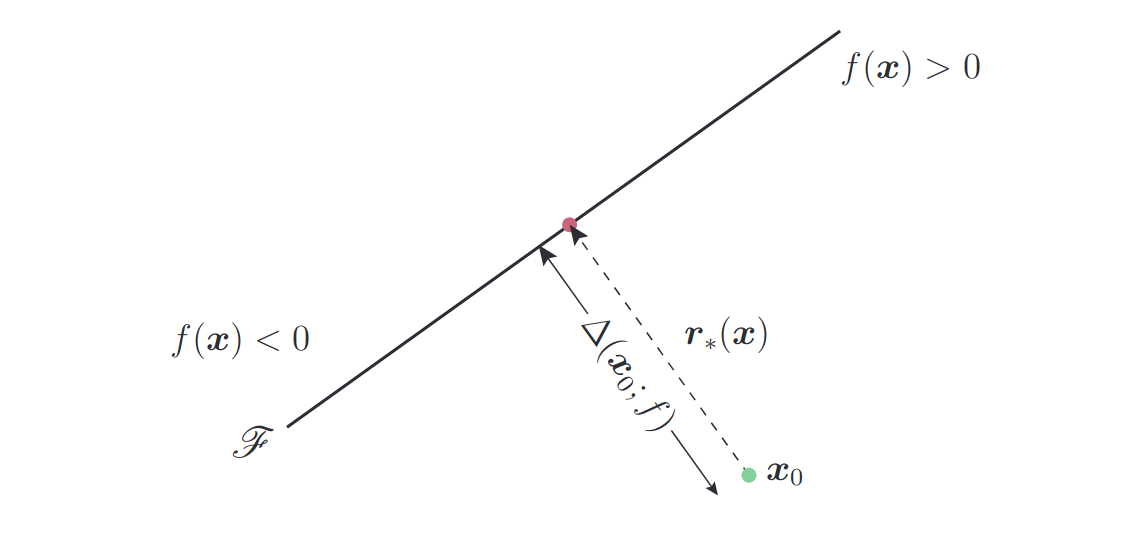
\includegraphics[width=\textwidth]{Images/DeepFool/Deepfool_1.png}
                \caption{Adversarial examples per un classificatore binario lineare}
                \label{DeepFool_1}
            \end{figure}\\
        
        La minima perturbazione è data da:
            \begin{equation}
                \begin{split}
                    r_*(x_0) :&= \operatorname*{arg\,min}_{sign(f(x_0+r)) \neq sign(f(x_0))} ||r||_2\\
                              &= -\frac{f(x_0)}{||w||_2^2}w
                \end{split}
            \end{equation}
            
        \newpage
        Di seguito è riportato l'algoritmo dell'attacco DeepFool per i classificatori binari:
            \begin{figure}[h!]
                \centering
                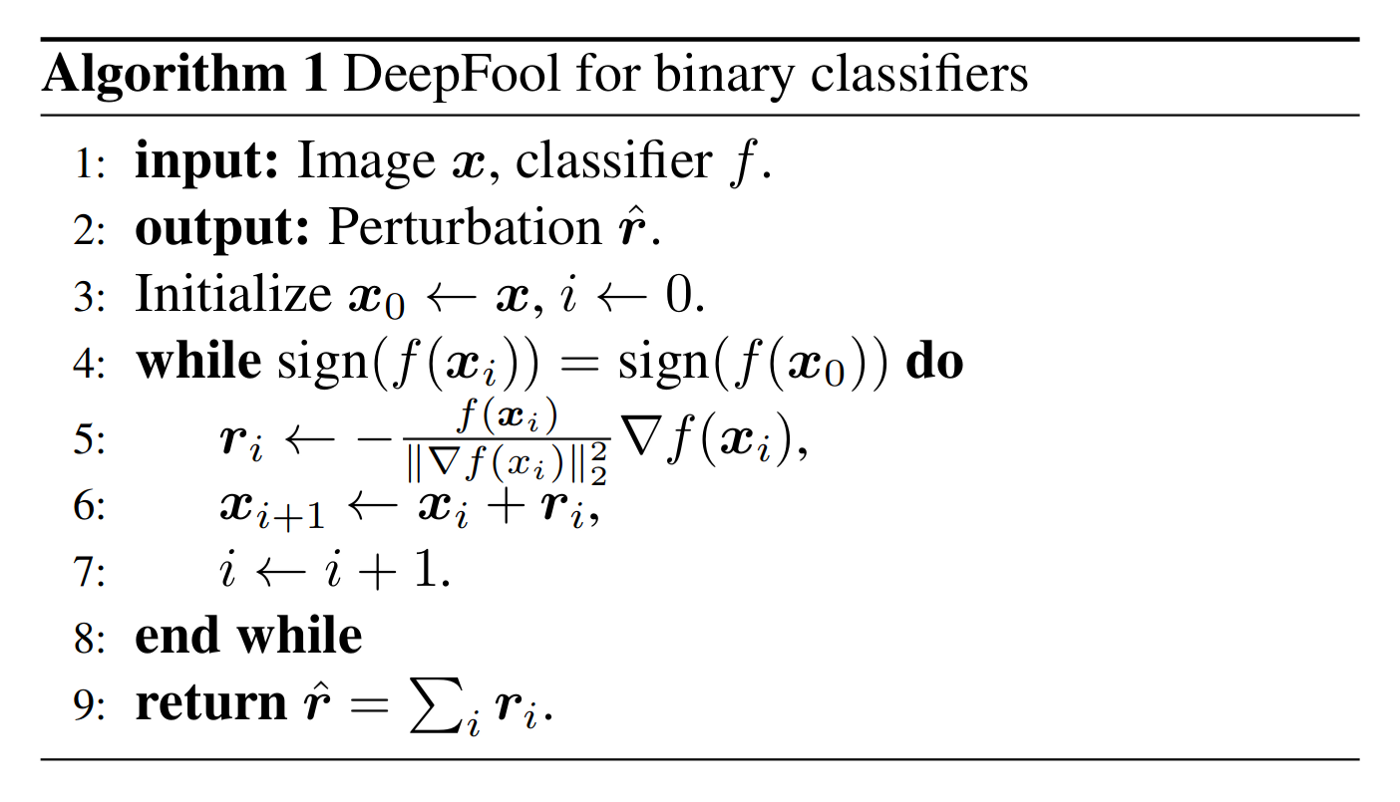
\includegraphics[width=0.8\textwidth]{Images/DeepFool/Deepfool_2.png}
                \caption{}
                \label{DeepFool_2}
            \end{figure}
            
            \paragraph{Analisi algoritmo}
                \begin{enumerate}
                    \item L'algoritmo prende in input $x$ e un classificatore $f$
                    \item Restituisce in output la perturbazione minima richiesta per classificare in modo errato l'immagine
                    \item Inizializza l'adversarial example con l'input originale. E la variabile $i$ del ciclo a 1.
                    \item Avviare il ciclo. Continuare il ciclo finché l'etichetta vera e l'etichetta dell'immagine perturbata avversariamente sono uguali.
                    \item Calcolare la perturbazione minima, ovvero la proiezione dell'input sull'iperpiano più vicino.
                    \item Aggiungere la perturbazione calcolata all'immagine e testare.
                    \item Incrementare la variabile del loop
                    \item Fine del loop.
                    \item Restituire la perturbazione minima.
                \end{enumerate}
            \newpage
        
        \subsubsection*{DeepFool per classificatori multiclasse}
        Moosavi-Dezfooli \cite{moosavi2015deepfool} descrivono un classificatore multiclasse come un insieme di classificatori binari.
        Per i classificatori multiclasse l'input è $x$ e per ogni classe c'è un iperpiano (piano rettilineo che divide una classe dalle altre) e, in base alla posizione che occupa nello spazio, $x$ viene classificato in una classe specifica.
        
        Ciò che fa l'algoritmo è trovare l'iperpiano più vicino, proiettare $x$ su quell'iperpiano e poi spingerlo oltre l'intersezione. In questo modo la classificazione di $x$ verrà sbagliata con la minima perturbazione possibile.\\
        
        Di seguito l'equazione per calcolare l'iperpiano più vicino:
            \begin{equation}
            \label{closest hyperplane}
                \hat{l}(x_0) = 
                \operatorname*{arg\,min}_{k \neq \hat{k}(x_0)} \frac{|f_k(x_0)-f_{\hat{k}(x_0)}(x_0)|}{||w_k-w_{\hat{k}(x_0)}||_2}
            \end{equation}
        dove: le varibiabili che cominciano con $f$ sono le etichette di classe, la variabili che cominciano con $w$ sono i gradienti, le variabili con $k$ come pedice sono per le classi con più probabilità dopo la classe reale, e le variabili con $\hat{k}(x_0)$ sono per la classe reale.\\
        
        Di seguito l'equazione per calcolare la perturbazione minima, ovvero il vettore che proietta l'input sull'iperpiano più vicino:
            \begin{equation}
            \label{minimal perturbation}
                r_*(x_0)=\frac{|f_{\hat{l}(x_0)}(x_0)-f_{\hat{k}(x_0)}(x_0)|}{||w_{\hat{l}(x_0)}-w_{\hat{k}(x_0)}||^2_2}(w_{\hat{l}(x_0)}-w_{\hat{k}(x_0)})
            \end{equation}\\
        
        Di seguito è riportato l'algoritmo dell'attacco DeepFool per i classificatori multiclasse:
            \begin{figure}[h!]
                \centering
                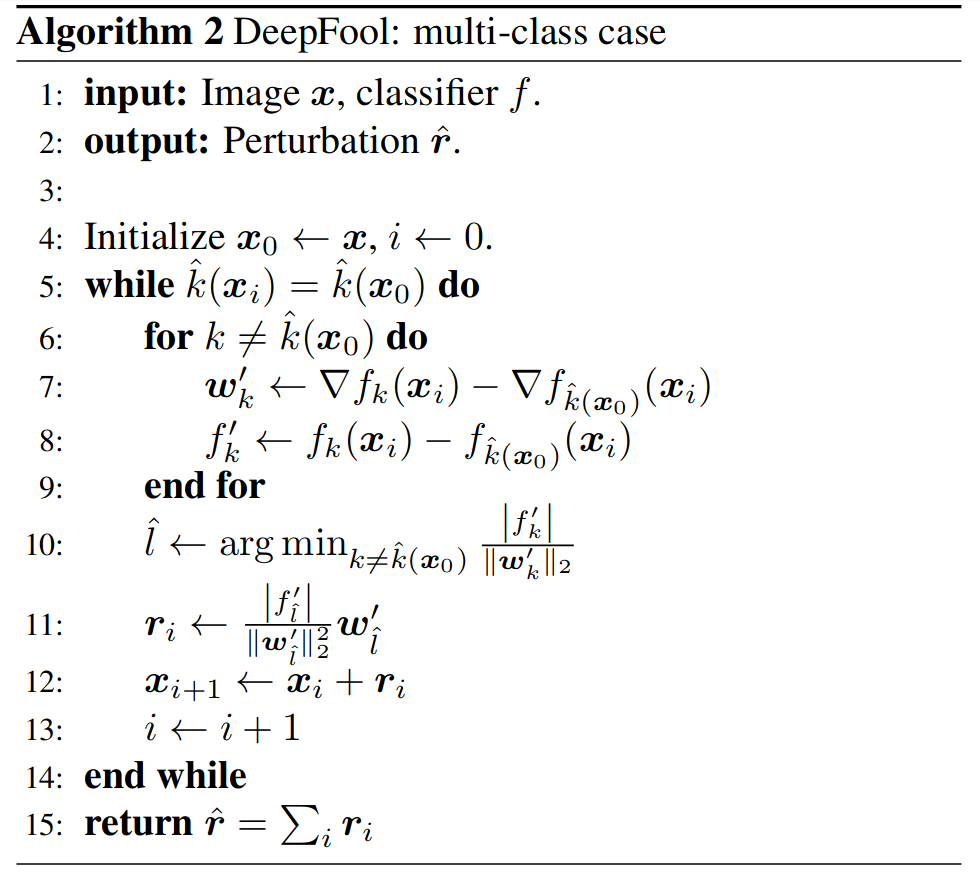
\includegraphics[width=0.7\textwidth]{Images/DeepFool/Deepfool_3.png}
                \caption{}
                \label{DeepFool_3}
            \end{figure}
        
            \paragraph{Analisi algoritmo}
                \begin{enumerate}
                    \item L'algoritmo prende in input $x$ e un classificatore $f$
                    \item Restituisce la perturbazione 
                    \item ...
                    \item Inizializza l'adversarial example con l'input originale. E la variabile $i$ del ciclo a 1.
                    \item Avviare il ciclo. Continuare il ciclo finché l'etichetta vera e l'etichetta dell'immagine perturbata sono uguali.
                    \item Si considerino n classi che hanno avuto una probabilità maggiore dopo la classe originale:
                    \item Memorizzare la differenza minima tra i gradienti originali e i gradienti di ciascuna di queste classi $w'_k$.
                    \item Memorizzare la differenza nelle etichette $f'_k$.
                    \item ...
                    \item Utilizzare $w'_k$ e $f'_k$ per calcolare l'iperpiano più vicino $\hat{l}$ per l'input $x$. Vedi formula \ref{closest hyperplane}
                    \item Calcolare il vettore minimo $r_i$ che proietta $x$ sull'iperpiano più vicino $\hat{l}$.\\
                    Vedi formula \ref{minimal perturbation}
                    \item Aggiungere la perturbazione minima all'immagine e controllare se è stata classificata in modo errato.
                    \item Incrementare la variabile del loop
                    \item Fine del loop.
                    \item Restituire la perturbazione totale, ovvero la somma di tutte le perturbazioni calcolate.
                \end{enumerate}
            \newpage
    
\section{Tecniche di Mitigation di Adversarial Attacks}
\label{C3: Mitigation}
    \begin{figure}[!h]
        \centering
        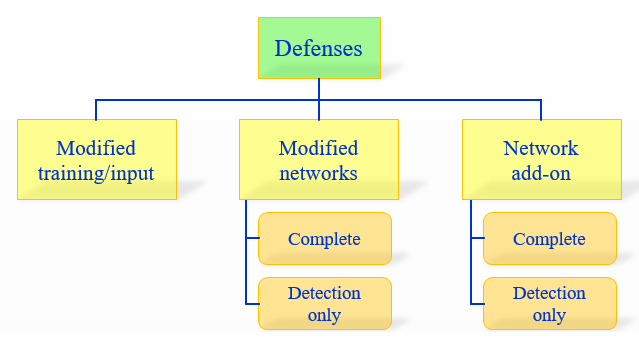
\includegraphics[width=0.8\textwidth]{Images/Mitigation/Defenses.png}
        \caption{Ampia categorizzazione di approcci volti a difendere le DNN dagli adversarial attacks.}
        \label{Defenses}
    \end{figure}
    Attualmente, le difese contro gli adversarial attacks si stanno sviluppando lungo 3 direzioni principali %[bibl: https://engineering.virginia.edu/sites/default/files/common/departments/electrical-and-computer-engineering/computer-engineering/files/Threat%20of%20Adversarial%20Attacks.pdf]
    \cite{akhtar2018threat}:
        \begin{enumerate}
            \item Modificare il metodo di apprendimento durante la fase di training o gli input durante la fase di testing.
            \item Modificare la rete, ad esempio aggiungendo più strati/sottoreti, cambiando loss function o activation function, ecc.
            \item Usando modelli esterni come network add-on quando si classificano esempi mai visti.
        \end{enumerate}
    Nel primo caso non ci si occupa direttamente del modello di apprendimento. Al contrario, le altre due categorie sono più incentrate sulle reti neurali stesse. In particolare:
        \begin{itemize}
            \item \textbf{Modifica di una rete}: si apportano modifiche all'architettura e/o ai parametri della rete neurale originale durante la fase di training.
            \item \textbf{Network add-on}: si mantiene il modello originale intatto e si aggiungono uno o più modelli esterni durante la fase di testing. Questi ultimi vengono utilizzati per preprocessare gli input prima che vengano passati al modello originale.
        \end{itemize}
    Le tecniche sotto queste categorie possono essere ulteriormente divise in due tipi: 
        \begin{itemize}
            \item \textbf{Complete defence} (Difesa completa): approccio che mira a permettere al modello attaccato di svolgere il suo compito originale anche sugli adversarial examples. Nel caso di un classificatore, ci si aspetta che il modello predica le classi degli adversarial examples con una precisione accettabile.
            \item \textbf{Detection only} (Solo rilevamento): approccio che mira ad individuare i potenziali adversarial examples, per poterli contrassegnare e rifiutare in qualsiasi elaborazione futura.
        \end{itemize}
    La gerarchia di queste categorie è mostrata nella figura \ref{Defenses}.
    Il resto della sezione è organizzato secondo questa gerarchia.
    \newpage
    
    \subsection{Modified Training/Input}
    \label{BF Adversarial Training}    
        \subsubsection{Brute-force adversarial training}
        L'adversarial training %[bibl: https://arxiv.org/pdf/1412.6572.pdf] 
        \cite{goodfellow2014explaining} è un metodo di difesa intuitivo contro gli adversarial attacks, che cerca di migliorare la robustezza di una rete neurale trainandola con adversarial examples.
        
        Formalmente, può essere formulato come segue:
            \begin{equation}
                \operatorname*{min}_{\theta} \operatorname*{max}_{D(x, x_{adv})<\eta}J(\theta,x_{adv},y)
            \end{equation}
        dove $J(\theta,x_{adv},y)$ è l'\textit{adversarial loss}, con \textit{weights} $\theta$, \textit{adversarial input} $x_{adv}$, e classe reale $y$. $D(x, x_{adv})$ è la distanza tra $x$ e $x_{adv}$.
        Il problema di massimizzazione interna è quello di trovare gli adversarial examples più efficaci ed è risolto da un adversarial attack ben progettato, come FGSM (\hyperref[FGSM]{\ref*{FGSM}}) e PGD (\hyperref[PGD]{\ref*{PGD}}).  
        La minimizzazione esterna è la procedura di addestramento standard per minimizzare la \textit{loss}. 
        
        Risolti i problemi di massimizzazione e minimizzazione, si suppone che la rete risultante sia resistente contro l'adversarial attack usato per la generazione di adversarial examples nella fase di training.
        
        Anche se l'adversarial training migliora la robustezza di una rete, è una strategia non adattativa che richiede che il training sia eseguito utilizzando attacchi forti e che l'architettura della rete sia sufficientemente rappresentativa.
        Inoltre, il metodo richiede un raddoppio della dimensione del Training dataset e, di conseguenza, un aumento di tempo e risorse investite nella fase di training.
            \begin{figure}[!h]
                \centering
                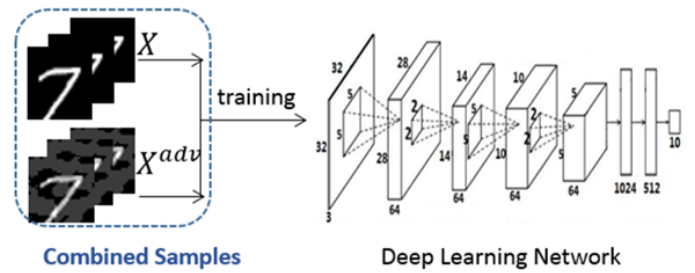
\includegraphics[width=0.8\textwidth]{Images/Mitigation/Adversarial training.png}
                \caption{Adversarial Training: trainare il modello con immagini pulite e perturbate}
                \label{Adversarial Training}
            \end{figure}
    \newpage
    
        \subsubsection{Random input transformation}
        In %[bibl: https://arxiv.org/pdf/1711.01991.pdf]
        \cite{xie2017mitigating} gli autori utilizzano due trasformazioni casuali per mitigare gli effetti degli adversarial attacks:
            \begin{enumerate}
                \item \textbf{Random resize}: ridimensionamento delle immagini di input ad una dimensione casuale prima di passarle alla rete neurale. 
                \item \textbf{Random padding}: riempimento con degli zeri intorno alle immagini di input in modo casuale.
            \end{enumerate}
        La pipeline di questo meccanismo rapido e preciso è mostrata nella figura \ref{Random resize and padding}
            \begin{figure} [!h]
                \centering 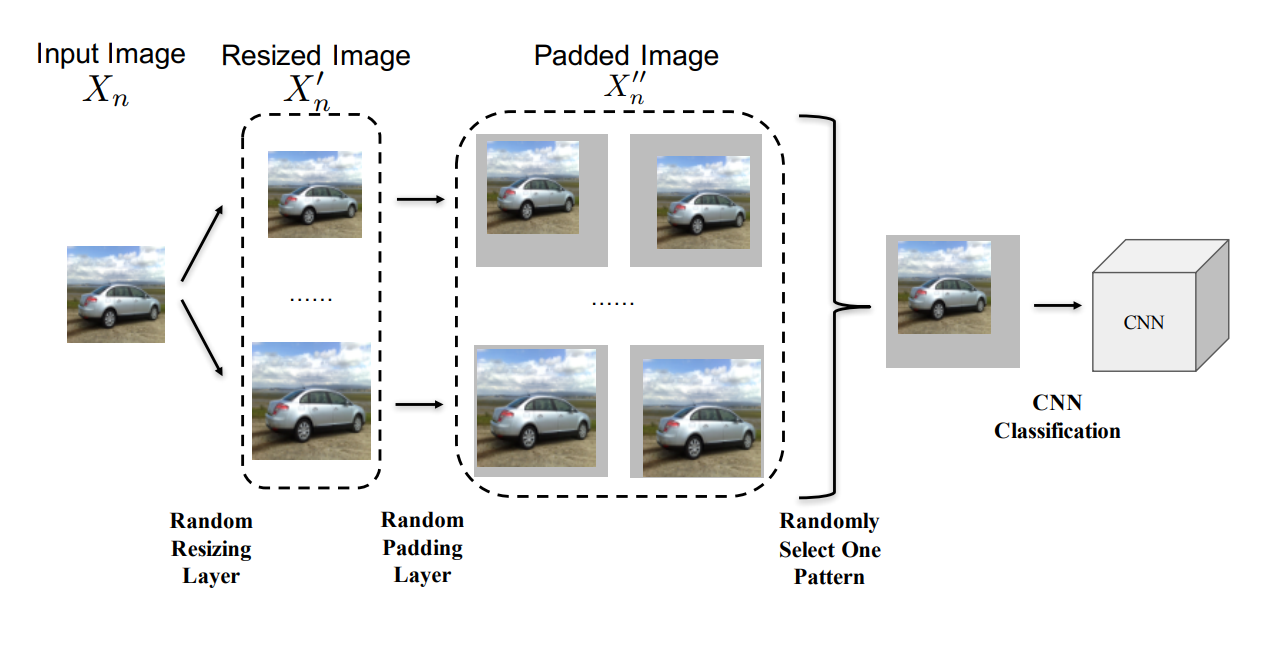
\includegraphics[width=\textwidth]{Images/Mitigation/Random resize and padding.png}
                \caption{Pipeline del meccanismo di difesa basato sulla randomizzazione. L'immagine in input $X_n$ passa attraverso il random resize layer che la scala in modo casuale. Poi, il random paddding layer applica il padding all'immagine ridimensionata $X'_n$ in maniera casuale. L'immagine risultante $X''_n$ viene utilizzata per la classificazione}
                \label{Random resize and padding}
            \end{figure}
    \newpage
    
    
    
    \subsection{Modified Networks}
        
        \subsubsection{Random noising}
        Random self-ensemble (RSE) %[bibl: https://arxiv.org/pdf/1712.00673v2.pdf]
        \cite{liu2017towards} è un algoritmo che aggiunge un noise layer dopo ogni convolutional layer in entrambe le fasi di training e testing, e raggruppa i risultati delle predizione per stabilizzare gli output della rete neurale, come mostrato nella Figura \ref{Random noising}.
        
        Lo stesso metodo può essere sviluppato utilizzando la differential privacy (DP). Il metodo PixelPD 
        %[bibl: https://ieeexplore.ieee.org/stamp/stamp.jsp?tp=&arnumber=8835364]
        \cite{lecuyer2018certified} include un DP noising layer all'interno della rete neurale per far rispettare i limiti DP sulla variazione della distribuzione sulle sue previsioni degli input con piccole perturbazioni basate sulle norme.
        
        Ispirandosi a PixelDP, Li %[bibl: https://proceedings.neurips.cc/paper/2019/file/335cd1b90bfa4ee70b39d08a4ae0cf2d-paper.pdf]
        \cite{li2018certified} propone inoltre di aggiungere direttamente del random noise ai pixel degli adversarial examples prima della classificazione, al fine di eliminare gli effetti delle perturbazioni avversarie.
            \begin{figure}[!h]
                \centering 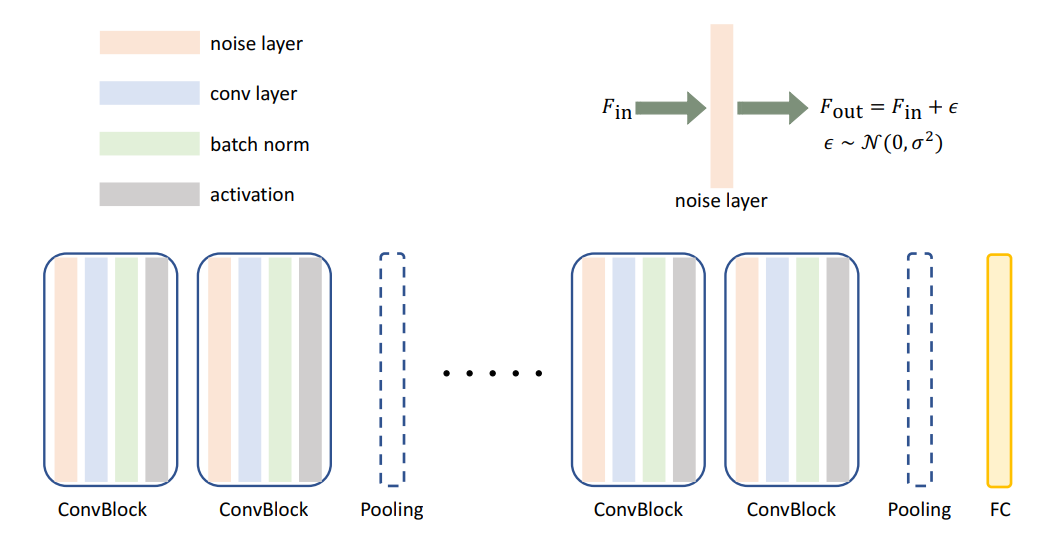
\includegraphics[width=0.8\textwidth]{Images/Mitigation/Random noising.png}
                \caption{Architettura di RSE. FC: fully connected layer; $F_in$: il vettore in input del noise layer; $F_out$: il vettore in output del noise layer; $\epsilon$: la perturbazione che segue la distribuzione gaussiana $\mathcal{N}(0, \sigma^2)$; conv: convolution}.
                \label{Random noising}
            \end{figure}
        
        \subsubsection{Gradient regularization/masking}
        In %[bibl: https://arxiv.org/pdf/1711.09404.pdf]
        \cite{ross2017improving} gli autori propongono un metodo che traina modelli differenziabili (ad esempio DNN) penalizzando il grado di variazione che risulta in output rispetto al cambiamento in input. Applicando una piccola perturbazione avversaria diventa improbabile che cambi drasticamente l'output del modello addestrato. 
        
        Si dimostra che questo metodo, quando combinato con il brute-force adversarial training, può garantire un'ottima robustezza alle reti neurali contro adversarial attacks come FGSM (\hyperref[FGSM]{\ref*{FGSM}}). 
        
        Tuttavia, ognuno di questi metodi quasi raddoppia la complessità di formazione di una rete, che risulta già proibitiva in molti casi.
    
    \newpage
    \subsection{Network Add-On}
    
        %\subsubsection{Feature Squeezing}
        %[bibl: https://arxiv.org/pdf/1704.01155.pdf] - molto vulnerabile, lo spiego comunque?
        
        \subsubsection{APE-GAN}
        Adversarial Perturbation Elimination GAN (APE-GAN) %[bibl: https://arxiv.org/pdf/1707.05474.pdf] 
        \cite{shen2017ape} ha l'obiettivo di mitigare l'adversarial attack agendo sull'input della rete neurale. 
        Sfrutta le proprietà delle GAN e la loro capacità di stimare la distribuzione dei campioni in input.
        
        APE-GAN è trainata in un ambiente avversario. Il suo Generator G, presa in input un'immagine perturbata, la restituisce in output pulita. Il suo Discriminator D confronta l'output del Generator con gli input reali puliti.
        
        In un ambiente ideale, il Generator impara a generare immagini pulite molto simili a quelle reali, rendendo difficile per il Discriminator predire la fonte delle sue immagini in input.
        \begin{figure}[!h]
            \centering
            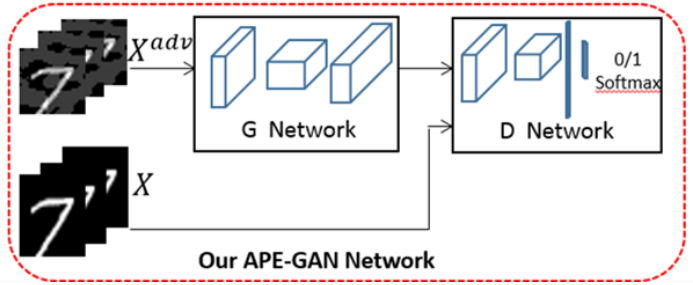
\includegraphics[width=0.6\textwidth]{Images/Mitigation/APE-GAN.png}
            \caption{APE-GAN: elimina la perturbazione dagli adversarial examples prima di passarli in input al modello originale per poterne incrementare la robustezza.}
            \label{APE-GAN}
        \end{figure}
        
        \subsubsection{Defense-GAN}
        Defense-GAN %[bibl: https://arxiv.org/pdf/1805.06605.pdf] 
        \cite{samangouei2018defense} si basa sulla tipica struttura delle WGAN %[bibl: https://arxiv.org/pdf/1701.07875.pdf]
        \cite{arjovsky2017wasserstein}. 
        
        Il Generator della Defense-GAN dovrebbe imparare a creare una mappatura da un vettore $z$ di bassa dimensione ad uno spazio di campioni di input di dimensione superiore.
        
        L'idea è di addestrare la Defence-GAN su dati originali e puliti che ci permettano di assumere con sicurezza che questi saranno vicini a qualche punto nell'intervallo di G. Ciò significa che gli adversarial examples saranno più lontani dall'intervallo di G. 
        
        Quindi, proiettare gli adversarial examples sull'intervallo del Generator si rivela un modo per diminuire le perturbazioni dalle immagini.
        
        Questo output proiettato viene dato in input alla rete neurale al posto degli adversarial examples.
            \begin{figure}[!h]
                \centering 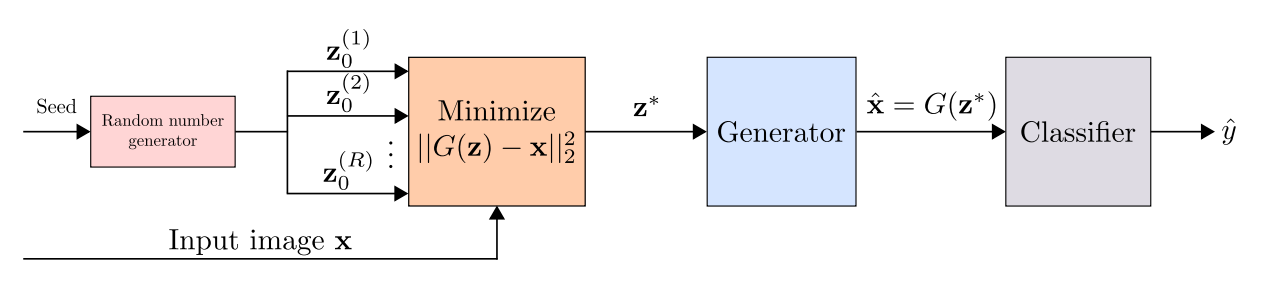
\includegraphics[width=0.9\textwidth]{Images/Mitigation/Defense-GAN.png}
                \caption{Panoramica dell'algoritmo Defense-GAN}
                \label{Defense-GAN}
            \end{figure}
        \newpage
        
        \subsubsection{MagNet}
        L'obiettivo di MagNet %[bibl: https://arxiv.org/pdf/1705.09064.pdf] 
        \cite{meng2017magnet} è quello di riconoscere gli adversarial examples.
        
        Se l'input è ritenuto pulito, MagNet lo trasforma ulteriormente con lo scopo di risolvere eventuali errori di classificazione del modello (figura \ref{MagNet}).
        
        L'architettura di MagNet consiste in un Detector e un Reformer. Entrambi possono essere costituiti da una o più reti concatenate.\\
        
        Sono stati proposti due Detectors:
            \begin{itemize}
                \item Il primo Detector sfrutta un AutoEncoder che viene trainato su campioni puliti e, quindi, impara a ricostruire le immagini appartenenti alla stessa distribuzione. Un adversarial example non apparterrà alla stessa distribuzione delle immagini pulite. Quindi, l'autoencoder trainato sulle immagini pulite avrà un'alta reconstruction loss nel caso di un adversarial example.
                \item Il primo Detector funziona bene con i campioni che hanno un elevato reconstruction error. Tuttavia non è necessario che un adversarial example abbia un elevato reconstruction error.
                
                Per questo motivo si decide di utilizzare il classificatore di destinazione. 
                
                Sia $f$ il classificatore e $ae$ l'autoencoder. Se un campione in input è perturbato, allora $f(x)$ e $f(ae(x))$ saranno molto diversi e avranno una divergenza grande.
                Si sfrutta quindi la divergenza di Jensen Shannon tra $f(x) e$ e $f(ae(x))$ per decidere se il campione in input è perturbato o pulito.
            \end{itemize}
        I Detectors sopra citati sono usati in serie con il Reformer 1 seguito dal Reformer 2. Se entrambi i Detectors ritengono l'input pulito, allora lo passano al Reformer 1:
            \begin{itemize}
                \item Reformer 1 basato sul random noise: aggiunge, all'immagine in input, un random noise basato su una distribuzione gaussiana standard. Lo svantaggio di questo reformer è che funziona allo stesso modo sia per un adversarial example che per un'immagine pulita.
                \item Reformer 2 basato su AutoEncoder: utilizza un autoencoder addestrato completamente su immagini pulite. Quando un adversarial example viene dato in input all'autoencoder, questo cercherà di ricostruire un'immagine pulita.
            \end{itemize}
        
            \begin{figure}[!h]
                \centering
                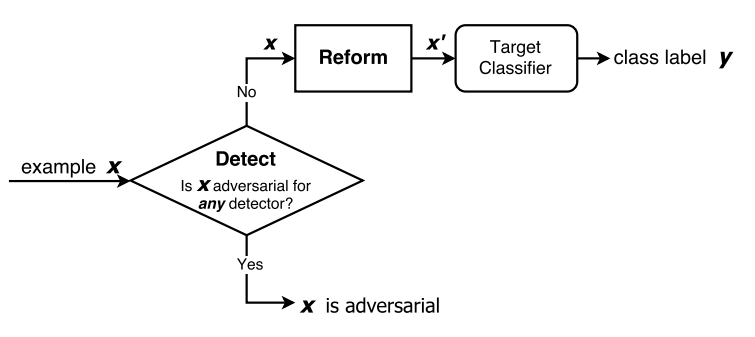
\includegraphics[width=0.7\textwidth]{Images/Mitigation/MagNet.png}
                \caption{Panoramica dell'algoritmo di MagNet}
                \label{MagNet}
            \end{figure}
    
        \subsubsection{Pix2Pix GAN}
        \label{Pix2Pix GAN}
        Una Pix2Pix GAN %[bibl: https://arxiv.org/pdf/1611.07004.pdf] 
        \cite{isola2016image} è una conditional GAN (cGAN) %[bibl: https://arxiv.org/pdf/1411.1784.pdf] 
        \cite{mirza2014conditional} ed utilizza solamente dati reali, rumore ed etichette per imparare a generare immagini.
        
        Uno dei campi in cui viene impiegata la Pix2Pix GAN è l'image denoising, ovvero, presa un'immagine che si presume perturbata con del rumore, si cerca di pulirla e riportarla allo stato originale.\\\\
        Il Generator impara la mappatura dai dati reali e dal rumore.
            \begin{equation*}
                G:\left \{ x, z \right \} \rightarrow y
            \end{equation*}
        Il Discriminator impara a la mappatura dalle etichette e dai dati reali.
            \begin{equation*}
                D(x, y)
            \end{equation*}
        Questa soluzione permette ad una cGAN di essere adatta a compiti di traduzione image-to-image, dove il Generator è vincolato ad un'immagine in input per generare un'immagine corrispondente in output. In altre parole, il Generator utilizza una condition distribution come una guida per generare un'immagine di destinazione. \\\\
        Pix2Pix GAN fonda la sua forza sulla fase di training, che consiste in una traduzione pair to pair image e il dataset utilizzato è composto da campioni di training {x, y} che hanno una corrispondenza tra loro. \\\\
        L'architettura di Pix2Pix GAN è composta da un Generator e un Discriminator:
            \begin{itemize}
                \item U-Net Generator %[bibl: https://arxiv.org/pdf/1505.04597.pdf]:
                      \cite{ronneberger2015u}:
                    \begin{figure}[!h]
                        \centering 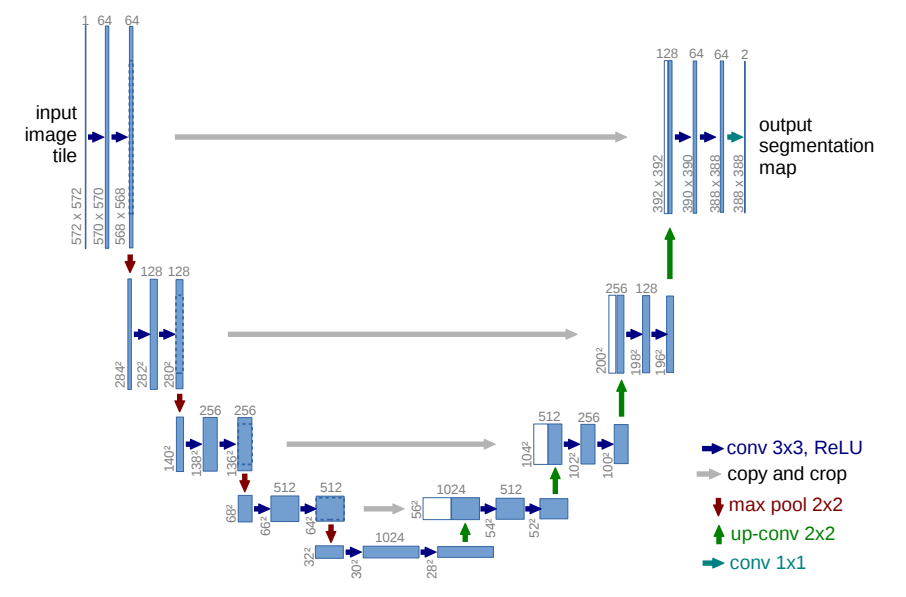
\includegraphics[width=0.8\textwidth]{Images/Mitigation/U-Net_1.png}
                        \caption{Architettura U-Net (esempio per immagini $32\times32$). \\
                        Ogni casella blu corrisponde ad una multi-channel feature map. Il numero di canali è indicato in cima al riquadro. La dimensione $x\times y$ è riportata sul bordo sinistro inferiore del riquadro.
                        I riquardi bianchi rappresentano feature maps copiate. 
                        Le frecce denotano le diverse operazioni.}
                        \label{U-Net_1}
                    \end{figure}
                \newpage
                
                U-Net si può dividere in due parti fondamentali (figura \ref{U-Net_2}):
                    \begin{enumerate}
                        \item Contracting path: è composto da convolutional layers (lato sinistro della figura \ref{U-Net_2}) che applicano un downsampling sui dati mentre estrae informazioni.
                        
                        Durante il downsampling, ogni convolutional block estrae delle informazioni parziali e le passa al convolutional block successivo per estratte ulteriori informazioni, fino a che non si raggiunge la parte centrale detta bottleneck.
                        \item Expansive path: è composto da transpose convolution layer (lato destro della figura \ref{U-Net_2}) che applica un upsampling sulle informazioni estratte in precedenza.
                        
                        L'upsampling comincia dal bottleneck.
                        Durante l'upsampling ogni transpose convolutional block espande le informazioni prese dal blocco precedente e le concatena a quelle estratte dal blocco corrente. Concatenando informazioni, U-Net può quindi imparare ad elaborare un output più preciso basandosi su queste informazioni.
                    \end{enumerate}
                    Il downsampling e l'upsampling devono avere lo stesso numero di convolution layer e transpose convolution layer. Questo perché bisognerà collegare i blocchi corrispondenti delle stesse dimensioni usando una skip connection.
                        \begin{figure}[!h]
                            \centering 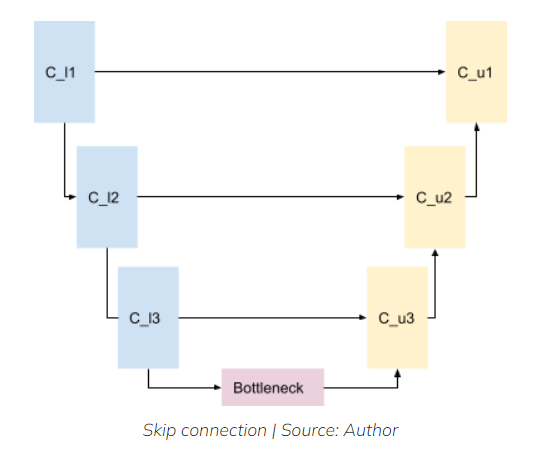
\includegraphics[width=0.7\textwidth]{Images/Mitigation/U-Net_2.png}
                            \caption{U-Net: contractive and expanding paths.}
                            \label{U-Net_2}
                        \end{figure}
                \newpage
                
                \item Markovian discriminator (PatchGAN):
                architettura contenente un certo numero di transpose convolutional blocks. Prende una porzione $N\times N$ dell'immagine e cerca di capire se è pulita o perturbata.
            
                $N$ può evere qualsiasi dimensione. $N$ può essere anche più piccolo dell'immagine originale, riuscirà comunque a produrre risultati di alta qualità.
                
                Seguendo questa procedura, il Discriminator viene applicato convoluzionalmente su tutta l'immagine. 
            \end{itemize}
        %L'equazione della loss function è la seguente ed ha due componenti, una per il Discriminator D e una per il Generator G:
        %    \begin{equation}
        %        \mathcal{L}_{cGAN}(G, D) = \mathbb{E}_{x,y}[log\, D(x, y)] + \mathbb{E}_{x,z}[log(1 - D(x, G(x, z))]
        %    \end{equation}
        
        %In ogni iterazione della fase di training della GAN il Discriminator è trainato prima del Generator in modo che possa riconoscere sia i dati reali che quelli generati dal Generator.
    \newpage

\chapter{Adversarial Attacks: esperimenti}
\label{chap:4}

In questo capitolo si illustrano due applicazioni di grande successo per la classificazione di immagini mediche:
\begin{enumerate}
    \item classificazione delle malattie del torace attraverso radiografie (chest X-Ray) del torace.
    \item classificazione delle malattie dell'encefalo attraverso risonanze magnetiche cerebrali.
\end{enumerate}
Inoltre, si descrivono alcune impostazioni sperimentali generali rispetto ai dataset e alle architetture di rete presi in esame durante il lavoro di tesi. \\\\
Infine, si riportano i risultati degli esperimenti condotti sugli attacchi scelti. 
\newpage

\section{Datasets}

    \subsection{Chest X-Ray (Pneumonia) Dataset}
        Dataset utilizzato per la classificazione delle malattie del torace attraverso radiografie (chest X-Ray) del torace.
        
        \paragraph{Cos'è la polmonite?}
        La polmonite è una malattia infiammatoria che può colpire uno o entrambi i polmoni.
        
        \paragraph{Perché è importante?} 
        Secondo l'Organizzazione Mondiale della Sanità (OMS), la polmonite uccide circa 2 milioni di bambini sotto i 5 anni ogni anno ed è costantemente stimata come la principale causa di mortalità infantile \cite{rudan2008epidemiology}, uccidendo più bambini di HIV/AIDS, malaria e morbillo messi insieme \cite{adegbola2012childhood}.
        
        Gli agenti patogeni batterici e virali sono le due principali cause di polmonite ma richiedono forme di gestione molto diverse.
        La polmonite batterica richiede un ricovero urgente per un trattamento antibiotico immediato, mentre la polmonite virale viene trattata con cure di supporto.
        
        Pertanto, una diagnosi accurata e tempestiva è imperativa per facilitare i ricoveri rapidi per i bambini che hanno bisogno di un intervento urgente. 
        
        \paragraph{Informazioni sul dataset}
        Il dataset \cite{Chest_X_Ray_Dataset} contiene 5863 immagini di radiografie di toraci di bambini suddivise in \textbf{2 classi}:
            \begin{itemize}
                \item \textbf{Normal}
                \item \textbf{Pneumonia} (o \textit{Polmonite}): ogni infiammazione, acuta o cronica del parenchima polmonare, causata principalmente da agenti patogeni batterici o virali.
            \end{itemize}
        
        Ad ogni immagine del dataset è assosciata una sola classe.\\\\
        Di seguito alcuni esempi di immagini contenute nel dataset:
            \begin{figure}[!ht]
                \centering
                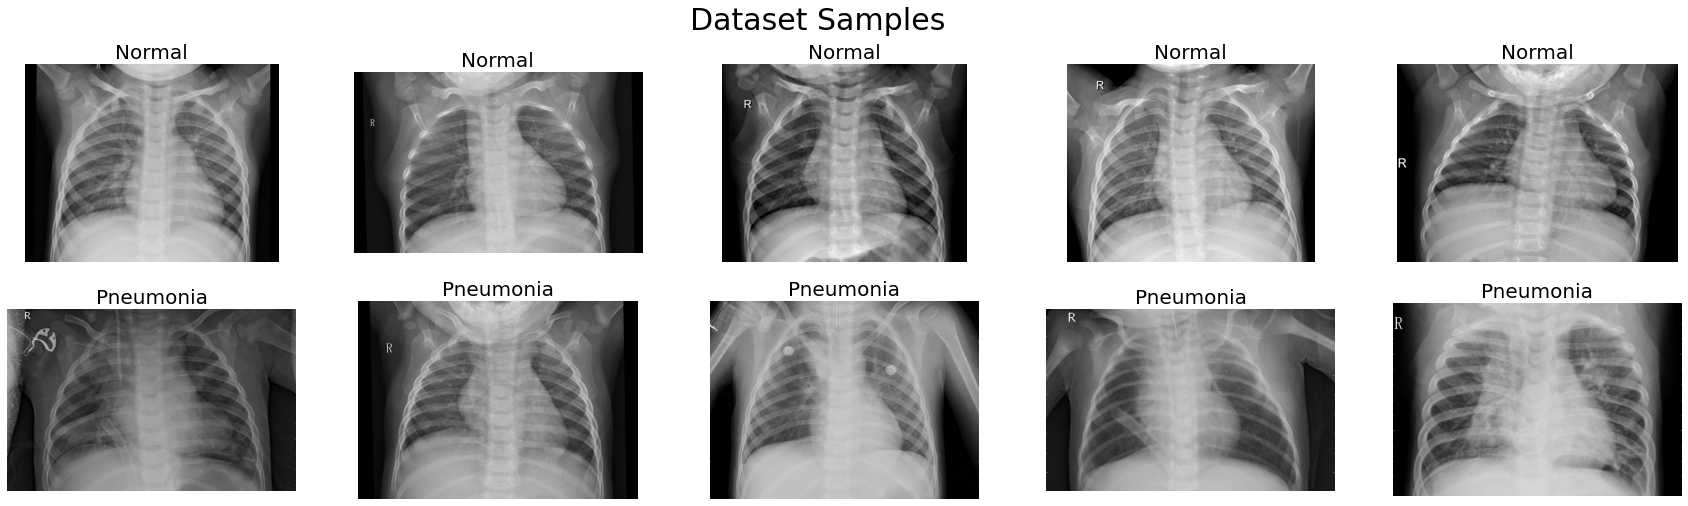
\includegraphics[width=\textwidth]{Images/Datasets/Pneumonia Dataset Samples.png}
                \caption{10 esempi di immagini presenti nel dataset \textit{Chest X-Ray}. I 5 esempi superiori aventi classe \textit{normal}, i 5 inferiori aventi classe \textit{pneumonia}.}
                \label{Pneumonia Samples}
            \end{figure}
    \newpage
    
    \subsection{Brain Tumor MRI Dataset}
        
        \paragraph{Cos'è un tumore cerebrale?}
        Un tumore al cervello è una massa di cellule, formatasi e cresciuta in modo del tutto anomalo all'interno dell'encefalo.
        
        I tumori al cervello, o tumori cerebrali, vengono classificati in base a più criteri, come la sede in cui comincia la crescita della massa tumorale e la velocità di diffusione (invasività) di quest'ultima.
        
        \paragraph{Perché è importante?}
        Il tumore al cervello è considerato una delle malattie più aggressive tra bambini e adulti. %\cite{Brain_Tumor_statistics}. 
        I tumori al cervello rappresentano l'85-90$\%$ di tutti i tumori primari del sistema nervoso centrale (SNC). Ogni anno, a circa 25.000 persone viene diagnosticato un tumore al cervello. Il tasso di sopravvivenza a 5 anni dalla diagnosi per le persone con un tumore al cervello o al SNC è di circa il 34$\%$ per gli uomini e il 36$\%$ per le donne.
        
        Trattamenti adeguati e ben pianificati, e una diagnosi accurata sono fondamentali per migliorare l'aspettativa di vita dei pazienti.
        
        La migliore tecnica per rilevare i tumori cerebrali è la risonanza magnetica (MRI). Un'enorme quantità di dati, sotto forma di immagini, viene generata attraverso le scansioni. Queste immagini vengono poi esaminate dai radiologi. Ma un esame manuale può essere soggetto ad errori a causa del livello di complessità dei tumori cerebrali e delle loro proprietà.
        
        L'applicazione di tecniche di classificazione automatizzata utilizzando l'apprendimento automatico (ML) e l'intelligenza artificiale (AI) ha dimostrato una maggiore accuratezza rispetto alla classificazione manuale.
        
        \paragraph{Informazioni sul dataset}
        Il dataset \cite{Brain_Tumor_MRI_Dataset} contiene 7022 immagini di risonanze magnetiche cerebrali umane suddivise in \textbf{4 classi}:
            \begin{itemize}
                \item \textbf{Glioma}: un tumore che si sviluppa a partire dalle cellule della glia (o cellule gliali) del sistema nervoso centrale.
                \item \textbf{Meningioma}: un tumore cerebrale che origina dalle meningi, ovvero le membrane protettive che circondano e proteggono il cervello e il midollo spinale.
                \item \textbf{No tumor}
                \item \textbf{Pituitary}: un adenoma ipofisario, anche conosciuto come adenoma pituitario, è un tumore generalmente benigno che colpisce l’ipofisi, una ghiandola dalle dimensioni molto ridotte che si trova sotto l’ipotalamo.
            \end{itemize}
        
        Ad ogni immagine del dataset è assosciata una sola classe.\\\\
        \newpage
        Di seguito alcuni esempi di immagini contenute nel dataset:
            \begin{figure}[!h]
                \centering
                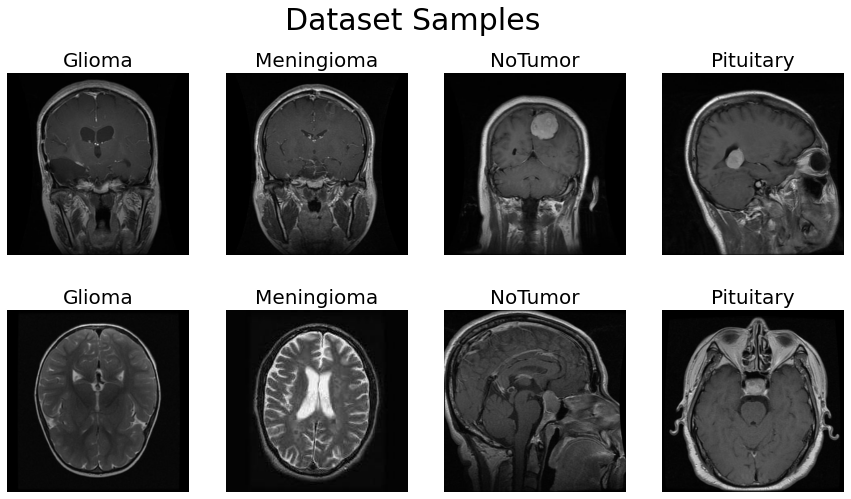
\includegraphics[width=\textwidth]{Images/Datasets/Brain Dataset Samples.png}
                \caption{8 esempi di immagini presenti nel dataset \textit{Brain Tumor MRI} con rispettive classi.}
                \label{Brain Samples}
            \end{figure}
        \newpage
        
    \subsection{Tecniche di Training}
            \paragraph{Hold-Out method}
            \label{Hold-Out method}
            Questo è il metodo utilizzato durante il lavoro di tesi.
            
            Il dataset viene diviso casualmente in 3 subdatasets seguendo le seguenti proporzioni:
                \begin{itemize}
                    \item Training dataset: $70\%$
                    \item Validation dataset: $20\%$
                    \item Testing dataset: $10\%$
                \end{itemize}
            
            \paragraph{Cross-validation method}
            
                \begin{itemize}
                    \item \textbf{k-fold method}: il dataset viene diviso casualmente in $k$ subdatasets di uguali dimensioni. Dei $k$ subdatasets solo uno viene scelto come Validation dataset, i restanti $k-$1 si concatenano per formare il Training dataset. Il processo viene ripetuto $k$ volte, con ciascuno dei $k$ subdatasets utilizzato solo una volta come Validation dataset.\\
                    Dopo aver calcolato i $k$ risultati finali si elabora la media per produrre una singola stima.\\
                    Comunemente si attribuisce $k=10$, ma in generale rimane un parametro non fissato. 
                        \begin{figure}[!h]
                            \centering
                            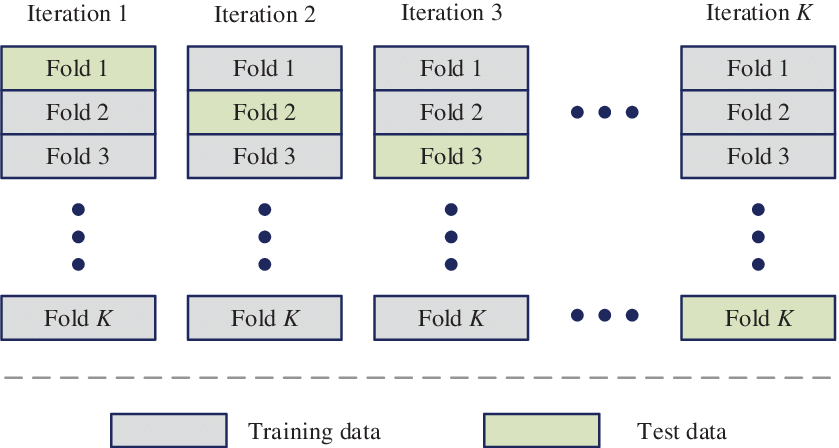
\includegraphics[width=0.7\textwidth]{Images/Datasets/K-fold-cross-validation-method.png}
                            \label{K-fold-cross-validation}
                            \caption{K-fold Cross-validation method}
                        \end{figure}
                    \item \textbf{n-fold method} (o \textbf{leave-one-out method}): Metodo simile al k-fold method.
                    Sia $n$ il numero di campioni all'interno del dataset, quest'ultimo viene diviso in $n$ subdatasets di dimensione 1, ognuno dei quali contiene uno e un solo campione del dataset.
                \end{itemize}
                
                Il vantaggio di questo metodo rispetto al \textit{Hold-Out method} è che tutti i campioni del dataset sono usati sia per il training che per la validation, e ogni campione è usato per la validation esattamente una volta. Per questo motivo il metodo aiuta a determinare una stima più accurata delle prestazioni di previsione del modello.
                Lo svantaggio è che il modello viene trainato $k$ volte e, in caso di datasets di dimensioni molto elevate, ciò può risultare estremamente costoso a livello computazionale.\\\\
            Durante il lavoro di tesi sono state provate entrambe le tecniche di training ma è stato scelto l'\textit{Hold-Out method} poiché, nonostante il \textit{k-fold cross-validation method} richieda un maggiore impiego di tempo e risorse a livello computazionale, non è stato in grado di ottenere un miglioramento significativo dei risultati.
                
\newpage        

\section{Modelli}

    \paragraph{Cos'è un modello pre-trainato e perché utilizzarlo}
    Un modello pre-trainato è un modello precedentemente trainato su un set di dati contenente \textit{weights} e \textit{biases} rappresentanti caratteristiche di quello specifico dataset. Se il dataset è abbastanza grande le caratteristiche apprese saranno molto probabilmente trasferibili su dataset differenti.
    
    L'utilizzo di un modello pre-trainato risulta vantaggioso perché permette di risparmiare tempo. Tempo e risorse di calcolo sono già state spese per permettere al modello di imparare caratteristiche fondamentali.\\
    
    Per il lavoro di tesi sono stati utilizzati 5 modelli CNN pre-trainati sul dataset ImageNet \cite{deng2009imagenet}, contenente più di 14 milioni di immagini divise in più di 20.000 classi:
        \begin{itemize}
            \item DenseNet121
            \item ResNet152 
            \item VGG19
            \item MobileNetV2
            \item InceptionV3
        \end{itemize}
    \newpage
    
    \subsection{DenseNet121}
    \label{DenseNet121}
    Una Dense Convolutional Network (DenseNet) %[bibl: https://arxiv.org/abs/1608.06993]
    \cite{huang2016densely}, collega ogni strato ad ogni altro strato in maniera feed forward. Mentre le reti convoluzionali tradizionali con L strati hanno L connessioni (una tra ogni strato e il suo successivo) una DenseNet ha L(L+1)/2 connessioni dirette. Per ogni strato, le feature-map di tutti gli strati precedenti sono usate come input, e le sue stesse feature-map sono usate come input in tutti gli strati successivi. 
    
    Le DenseNets hanno diversi vantaggi: alleviano il problema del vanishing-gradient, migliorano la propagazione delle features, incoraggiano il riutilizzo delle features e riducono sostanzialmente il numero di parametri.
        
        \paragraph{Architettura}
        Di seguito l'architettura del modello DenseNet121:
            \begin{table}[!h]
                \centering
                \begin{tabular}{|c|c|c|}
                    \hline 
                    \rule[-3mm]{0mm}{8mm}
                    \textbf{Layers} & \textbf{Output Size} & \textbf{DenseNet-121} \\
                    \hline \hline
                    \rule[-3mm]{0mm}{8mm}
                    Convolution & 112 $\times$ 112 & 7 $\times$ 7 conv, stride 2 \\
                    \hline 
                    \rule[-3mm]{0mm}{8mm}
                    Pooling & 56 $\times$ 56 & 3 $\times$ 3 max pool, stride 2\\
                    \hline 
                    \rule[-6mm]{0mm}{1.4cm}
                    Dense Block  (1) & 56 $\times$ 56 & $\begin{bmatrix} 1 \times 1  \hspace{.2cm} \text{conv}\\ 3 \times 3 \hspace{.2cm} \text{conv} \end{bmatrix} \times 6 $ \\
                    \hline
                    \rule[-3mm]{0mm}{8mm}
                    Transition Layer (1) & 56 $\times$ 56 & 1 $\times$ 1 conv \\
                    \cline{2-3}
                    \rule[-3mm]{0mm}{8mm}
                    & 28 $\times$ 28 & 2 $\times$ 2 avarage pool, stride 2\\
                    \hline 
                    \rule[-6mm]{0mm}{1.4cm}
                    Dense Block  (2) & 28 $\times$ 28 & $\begin{bmatrix} 1 \times 1  \hspace{.2cm} \text{conv}\\ 3 \times 3 \hspace{.2cm} \text{conv} \end{bmatrix} \times 12 $ \\
                    \hline
                    \rule[-3mm]{0mm}{8mm}
                    Transition Layer (2) & 28 $\times$ 28 & 1 $\times$ 1 conv \\
                    \cline{2-3}
                    \rule[-3mm]{0mm}{8mm}
                    & 14 $\times$ 14 & 2 $\times$ 2 avarage pool, stride 2\\
                    \hline 
                    \rule[-6mm]{0mm}{1.4cm}
                    Dense Block  (3) & 14 $\times$ 14 & $\begin{bmatrix} 1 \times 1  \hspace{.2cm} \text{conv}\\ 3 \times 3 \hspace{.2cm} \text{conv} \end{bmatrix} \times 24 $ \\
                    \hline
                    \rule[-3mm]{0mm}{8mm}
                    Transition Layer (3) & 14 $\times$ 14 & 1 $\times$ 1 conv \\
                    \cline{2-3}
                    \rule[-3mm]{0mm}{8mm}
                    & 7 $\times$ 7 & 2 $\times$ 2 avarage pool, stride 2\\
                    \hline 
                    \rule[-6mm]{0mm}{1.4cm}
                    Dense Block  (4) & 7 $\times$ 7 & $\begin{bmatrix} 1 \times 1  \hspace{.2cm} \text{conv}\\ 3 \times 3 \hspace{.2cm} \text{conv} \end{bmatrix} \times 16 $ \\
                    \hline
                    \rule[-3mm]{0mm}{8mm}
                    Classification Layer & 1 $\times$ 1 & 7 $\times$ 7 global avarage pool \\
                    \cline{2-3}
                    \rule[-3mm]{0mm}{8mm}
                    &  & 1000D fully-connected, softmax\\
                    \hline
                \end{tabular}
                \label{DenseNet121 Architecture}
            \end{table}
        
        \newpage
        
        \paragraph{Training and Validation Phase} 
        Di seguito sono riportati i grafici, prodotti durante il lavoro di tesi, raffiguranti le performance del modello, ovvero i valori dell'\textbf{accuracy} e della \textbf{loss} in funzione delle epoche, sia per la fase di \textit{Training} che di \textit{Validation}:
            \begin{figure}[!h]
                \centering
                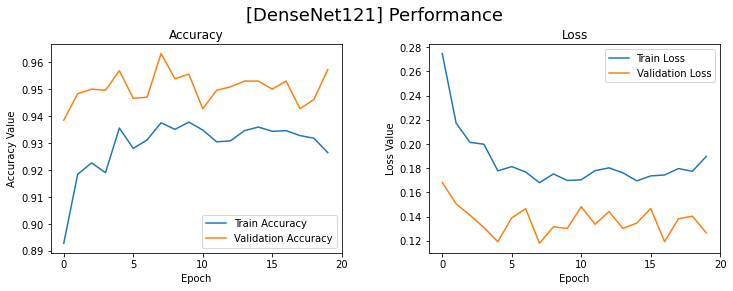
\includegraphics [width=\textwidth]{Images/Modelli/DenseNet121/DenseNet121 Pneumonia Performance.png}
                \caption{Performance durante le fasi di \textit{Training} e \textit{Validation} del modello \textit{DenseNet121} sui Training e Validation datasets di \textit{Chest X-Ray}}
                \label{DenseNet121 Pneumonia Performance}
            \end{figure}
            
            \begin{figure}[!h]
                \centering
                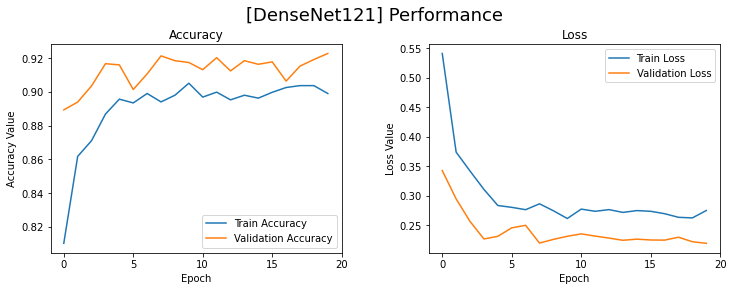
\includegraphics [width=\textwidth]{Images/Modelli/DenseNet121/DenseNet121 Brain Performance.png}
                \caption{Performance durante le fasi di \textit{Training} e \textit{Validation} del modello \textit{DenseNet121} sui Training e Validation datasets di \textit{Brain Tumor MRI}}
                \label{DenseNet121 Brain Performance}
            \end{figure}
        
        \newpage
        
        \paragraph{Testing Phase}
        Di seguito si riportano le Confusion Matrices e alcuni esempi di predizioni rispetto alle classi reali delle immagini, prodotti durante il lavoro di tesi:
            \begin{figure}[!h]
                \centering
                \subfloat[][Confusion Matrix del modello \textit{DenseNet121} sul Testing dataset di \textit{Chest X-Ray}] {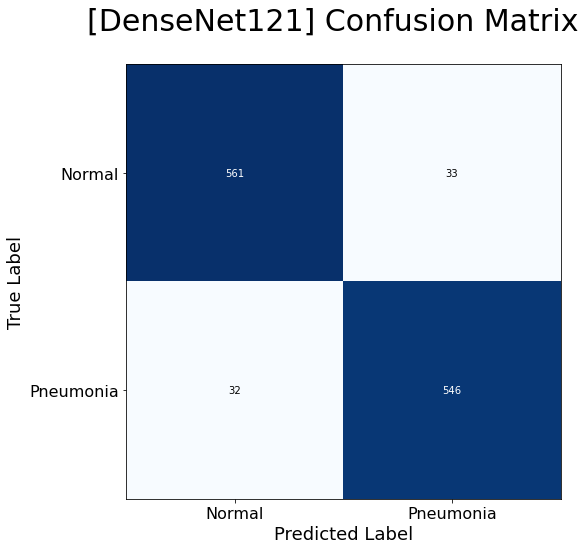
\includegraphics[width=.35\textwidth]{Images/Modelli/DenseNet121/DenseNet121 Pneumonia Confusion Matrix.png}} 
                \quad
                \subfloat[][Confusion Matrix del modello \textit{DenseNet121} sul Testing dataset di \textit{Brain Tumor MRI}] {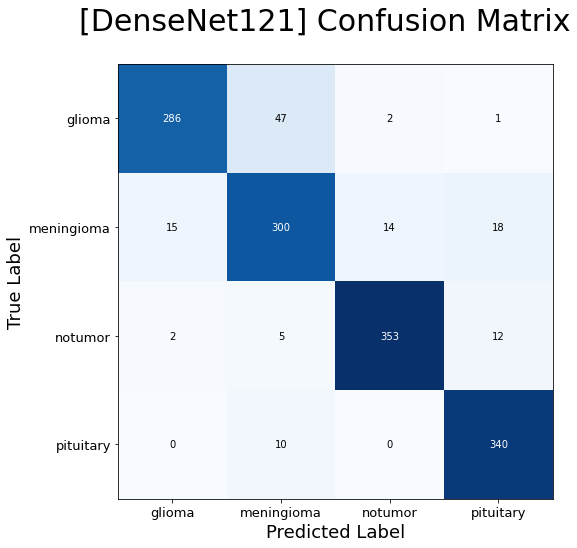
\includegraphics[width=.35\textwidth]{Images/Modelli/DenseNet121/DenseNet121 Brain Confusion Matrix.png}}
                \quad
                \subfloat[][10 esempi con rispettive classi reali e predizioni del modello \textit{DenseNet121} su immagini pulite del Testing dataset di \textit{Chest X-Ray}] {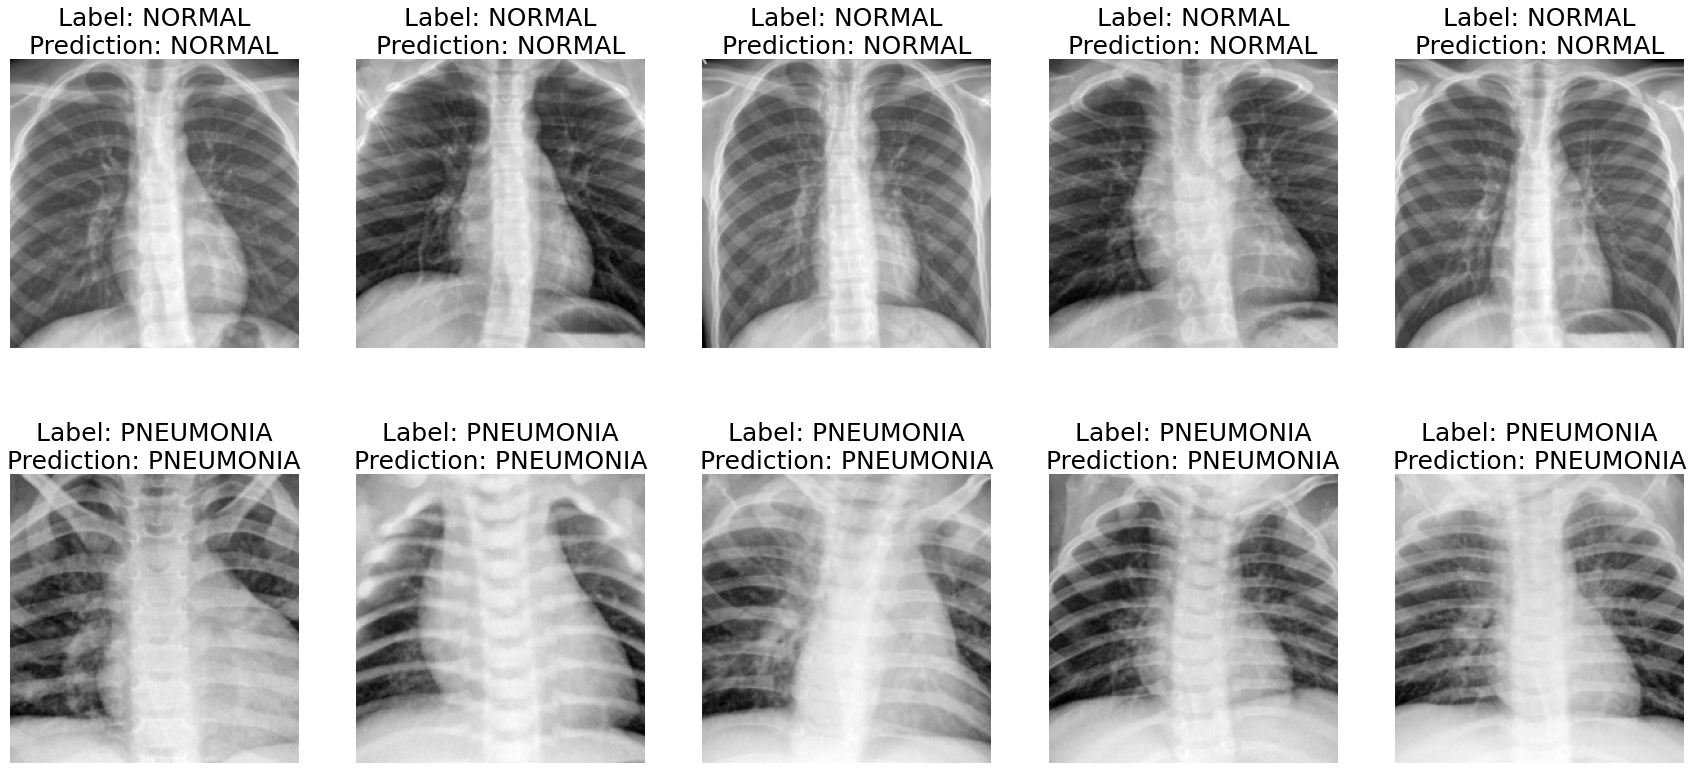
\includegraphics[width=.75\textwidth]{Images/Modelli/DenseNet121/DenseNet121 Pneumonia 10 True&Predictions.png}} \quad
                \subfloat[][8 esempi con rispettive classi reali e predizioni del modello\\ \textit{DenseNet121} su immagini pulite del Testing dataset di \textit{Brain Tumor MRI}] {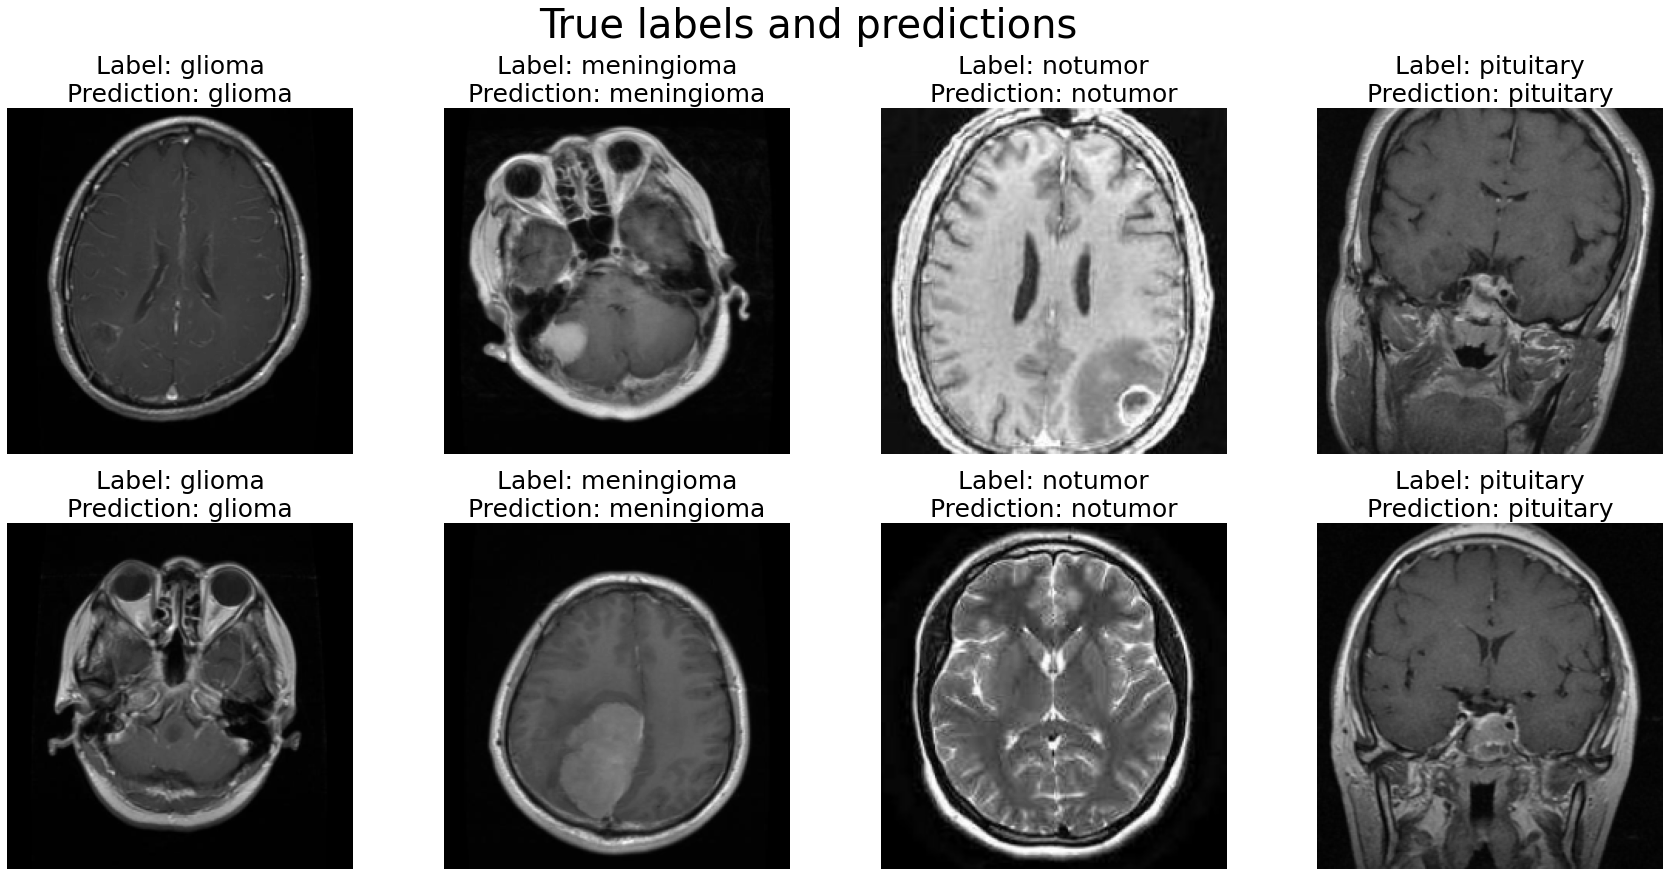
\includegraphics[width=.75\textwidth]{Images/Modelli/DenseNet121/DenseNet121 Brain 8 True&Predictions.png}}
                \caption{}
                \label{DenseNet121 Confusion Matrix and Predictions}
            \end{figure}
        \newpage
   
    \subsection{ResNet152}
    \label{ResNet152} 
    Una Residual Network (ResNet) \cite{he2015deep} limita la perdita di gradiente negli strati più profondi aggiungendo una connessione residua tra ogni strato di convoluzione.
        \begin{figure}[!h]
            \centering
            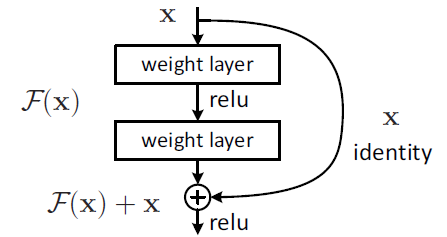
\includegraphics[width=0.5\textwidth]{Images/Modelli/ResNet152/Residual Connection.png}
            \caption{Residual Connection}
            \label{Residual Connection}
        \end{figure}
    
        \paragraph{Architettura}
        Di seguito l'architettura del modello ResNet152:
            \begin{table}[!h]
                \centering
                \begin{tabular}{|c|c|c|}
                \hline
                \rule[-3mm]{0mm}{8mm}
                \textbf{Layers}  & \textbf{Output Size} & \textbf{ResNet152} \\
                \hline \hline
                \rule[-3mm]{0mm}{8mm}
                conv 1 & 112 $\times$ 112 & 7 $\times$ 7, 64, stride 2 \\
                \hline
                \rule[-3mm]{0mm}{8mm}
                & & 3 $\times$ 3 max pool, stride 2\\
                \cline{3-3}
                \rule[-8mm]{0mm}{1.8cm}
                conv 2\textunderscore x & 56 $\times$ 56 &  $\begin{bmatrix} 1 \times 1, 64 \\  3 \times 3,  64 \\ 1 \times 1,  256 \end{bmatrix} \times 3 $ \\
                \hline
                \rule[-8mm]{0mm}{1.8cm}
                conv 3\textunderscore x & 28 $\times$ 28 &  $\begin{bmatrix} 1 \times 1, 128 \\  3 \times 3,  128 \\ 1 \times 1,  512 \end{bmatrix} \times 8 $ \\
                \hline
                \rule[-8mm]{0mm}{1.8cm}
                conv 4\textunderscore x & 14 $\times$ 14 &  $\begin{bmatrix} 1 \times 1, 256 \\  3 \times 3,  256 \\ 1 \times 1,  1024 \end{bmatrix} \times 36 $ \\
                \hline
                \rule[-8mm]{0mm}{1.8cm}
                conv 5\textunderscore x & 7 $\times$ 7  &  $\begin{bmatrix} 1 \times 1, 512 \\  3 \times 3,  512 \\ 1 \times 1,  2048 \end{bmatrix} \times 3 $ \\
                \hline
                \rule[-3mm]{0mm}{8mm}
                & 1 $\times$ 1 & average pool, 1000-d fc, softmax\\
                \hline
                \multicolumn{2}{|c|}{FLOPs} & \rule[-3mm]{0mm}{8mm}$11.3 \times 10^9$\\
                \hline
                \end{tabular}
               \label{ResNet152 Architecture}
            \end{table}
        \newpage
        
        \paragraph{Training and Validation Phase} 
        Di seguito sono riportati i grafici, prodotti durante il lavoro di tesi, raffiguranti le performance del modello, ovvero i valori dell'\textbf{accuracy} e della \textbf{loss} in funzione delle epoche, sia per la fase di \textit{Training} che di \textit{Validation}:
            \begin{figure}[!h]
                \centering
                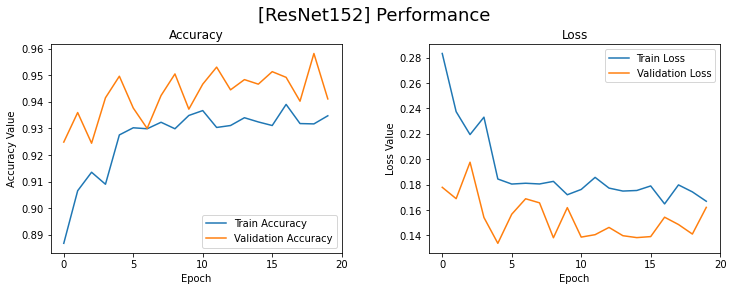
\includegraphics[width=0.7\textwidth]{Images/Modelli/ResNet152/ResNet152 Pneumonia Performance.png}
                \caption{Performance durante le fasi di \textit{Training} e \textit{Validation} del modello \textit{ResNet152} sui Training e Validation datasets di \textit{Chest X-Ray}}
                \label{ResNet152 Pneumonia Performance}
            \end{figure}
            
            \begin{figure}[!h]
                \centering
                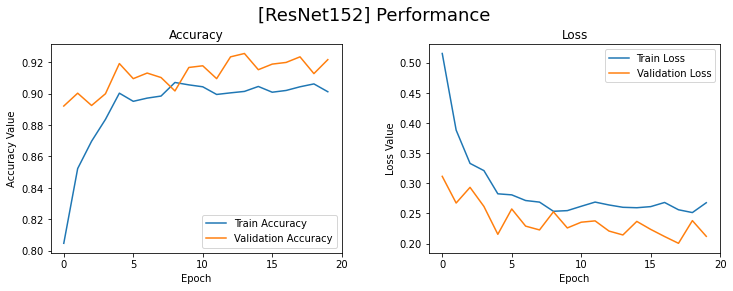
\includegraphics [width=0.7\textwidth]{Images/Modelli/ResNet152/ResNet152 Brain Performance.png}
                \caption{Performance durante le fasi di \textit{Training} e \textit{Validation} del modello \textit{ResNet152} sui Training e Validation datasets di \textit{Brain Tumor MRI}}
                \label{ResNet152 Brain Performance}
            \end{figure}
        
        \paragraph{Testing Phase}
        Di seguito si riportano le Confusion Matrices prodotte durante il lavoro di tesi:
            \begin{figure}[!h]
                \centering
                \subfloat[][Confusion Matrix del modello \textit{ResNet152} sul Testing dataset di \textit{Chest X-Ray}] {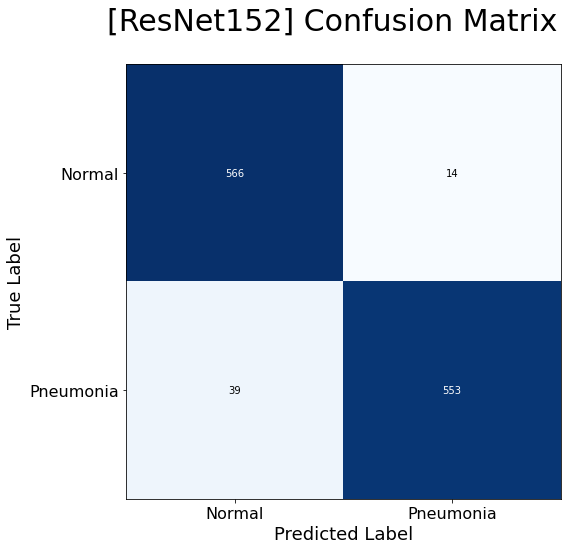
\includegraphics[width=.3\textwidth]{Images/Modelli/ResNet152/ResNet152 Pneumonia Confusion Matrix.png}} 
                \quad
                \subfloat[][Confusion Matrix del modello \textit{ResNet152} sul Testing dataset di \textit{Brain Tumor MRI}] {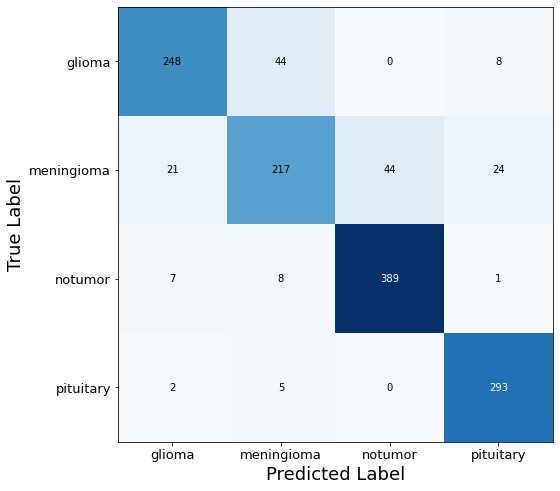
\includegraphics[width=.3\textwidth]{Images/Modelli/ResNet152/ResNet152 Brain Confusion Matrix.png}}
                \caption{}
                \label{ResNet152 Confusion Matrix}
            \end{figure}
        \newpage 
    
    \subsection{VGG19}
    \label{VGG19}
    
    %[bibl: arXiv:1409.1556]
    
        \paragraph{Architettura}
        Di seguito l'architettura del modello VGG19 \cite{simonyan2014very}:\\
            \begin{table} [!h]
                \centering
                \begin{tabular}{|c|}
                    \hline 
                    ConvNet Configuration\\
                    \hline \hline
                    \rule[-3mm]{0mm}{8mm}
                    \textbf{19 weight layers}\\
                    \hline
                    \hline
                    \rule[-3mm]{0mm}{8mm}
                    input ($224\times224$ RGB image)\\
                    \hline
                    conv3-64\\
                    conv3-64\\
                    \hline 
                    \rule[-3mm]{0mm}{8mm}
                    maxpool (1)\\
                    \hline 
                    conv3-128\\
                    conv3-128\\
                    \hline  
                    \rule[-3mm]{0mm}{8mm}
                    maxpool (2)\\
                    \hline 
                    conv3-256\\
                    conv3-256\\
                    conv3-256\\
                    conv3-256\\
                    \hline 
                    \rule[-3mm]{0mm}{8mm}
                    maxpool (3)\\
                    \hline 
                    conv3-512\\
                    conv3-512\\
                    conv3-512\\
                    conv3-512\\
                    \hline 
                    \rule[-3mm]{0mm}{8mm}
                    maxpool (4)\\
                    \hline 
                    conv3-512\\
                    conv3-512\\
                    conv3-512\\
                    conv3-512\\
                    \hline 
                    \rule[-3mm]{0mm}{8mm}
                    maxpool (5)\\
                    \hline 
                    \rule[-3mm]{0mm}{8mm}
                    FC-4096\\
                    \hline 
                    \rule[-3mm]{0mm}{8mm}
                    FC-4096\\
                    \hline 
                    \rule[-3mm]{0mm}{8mm}
                    FC-1000\\
                    \hline 
                    \rule[-3mm]{0mm}{8mm}
                    soft-max\\
                    \hline 
                \end{tabular}
            \end{table}
        \newpage
        
        \paragraph{Training and Validation Phase} 
        Di seguito sono riportati i grafici, prodotti durante il lavoro di tesi, raffiguranti le performance del modello, ovvero i valori dell'\textbf{accuracy} e della \textbf{loss} in funzione delle epoche, sia per la fase di \textit{Training} che di \textit{Validation}:
            \begin{figure}[!h]
                \centering
                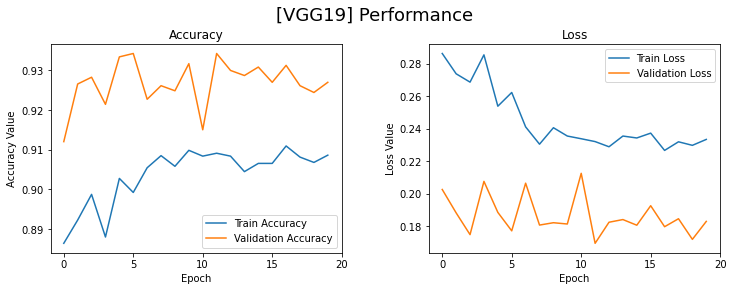
\includegraphics[width=0.7\textwidth]{Images/Modelli/VGG19/VGG19 Pneumonia Performance.png}
                \caption{Performance durante le fasi di \textit{Training} e \textit{Validation} del modello \textit{VGG19} sui Training e Validation datasets di \textit{Chest X-Ray}}
                \label{VGG19 Pneumonia Performance}
            \end{figure}
            
            \begin{figure}[!h]
                \centering
                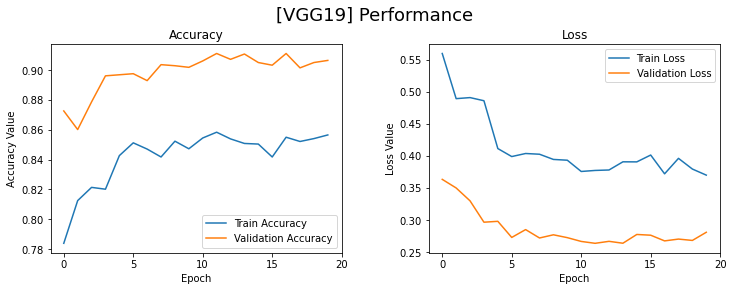
\includegraphics [width=0.7\textwidth]{Images/Modelli/VGG19/VGG19 Brain Performance.png}
                \caption{Performance durante le fasi di \textit{Training} e \textit{Validation} del modello \textit{VGG19} sui Training e Validation datasets di \textit{Brain Tumor MRI}}
                \label{VGG19 Brain Performance}
            \end{figure}
        
        \paragraph{Testing Phase}
        Di seguito si riportano le Confusion Matrices prodotte durante il lavoro di tesi:
            \begin{figure}[!h]
                \centering
                \subfloat[][Confusion Matrix del modello \textit{VGG19} sul Testing dataset di \textit{Chest X-Ray}] {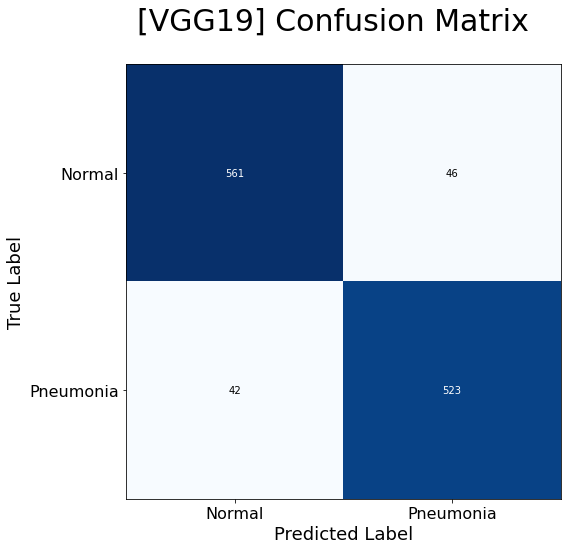
\includegraphics[width=.3\textwidth]{Images/Modelli/VGG19/VGG19 Pneumonia Confusion Matrix.png}} 
                \quad
                \subfloat[][Confusion Matrix del modello \textit{VGG19} sul Testing dataset di \textit{Brain Tumor MRI}] {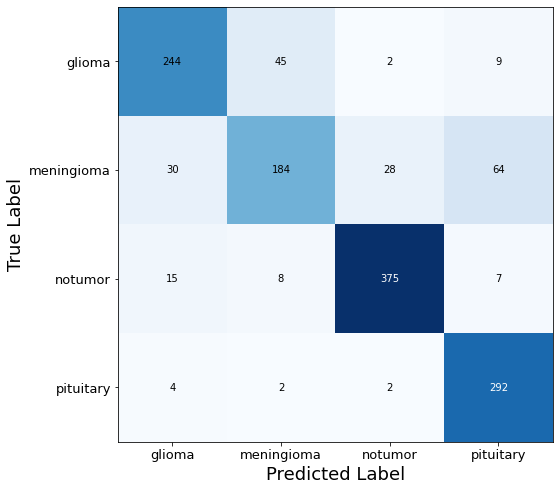
\includegraphics[width=.3\textwidth]{Images/Modelli/VGG19/VGG19 Brain Confusion Matrix.png}}
                \caption{}
                \label{VGG19 Confusion Matrix}
            \end{figure}
        \newpage 
       
    \subsection{MobileNetV2}
    \label{MobileNetV2}
    Il modello MobileNetV2 %[bibl: arXiv:1801.04381] 
    \cite{sandler2018mobilenetv2} è basato su una struttura \textit{inverted residual} in cui l'input e l'output del \textit{residual block} sono sottili\textit{ bottleneck layers}, al contrario dei \textit{residual models} tradizionali che usano in input \textit{expanded representations}.
    MobileNetV2 utilizza leggere \textit{depthwise convolutions} per filtrare le \textit{features} nel \textit{expansion layer }intermedio.
        \begin{figure}[!h]
            \centering
            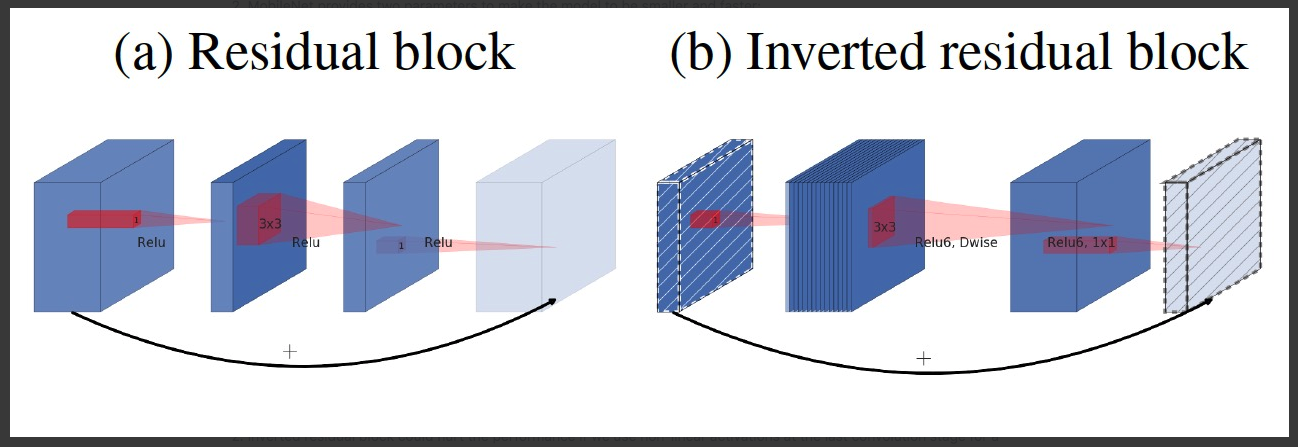
\includegraphics[width=0.6\textwidth]{Images/Modelli/MobileNetV2/Inverted residual block.png}
            \label{MobileNetV2 blocks}
        \end{figure}
        
        \paragraph{Standard residual block}
        Uno\textit{ standard residual block} comprime i canali larghi in canali stretti con convoluzioni $1\times1$ e $3\times3$, e poi li espande di nuovo in canali larghi con convoluzioni $1\times1$.
        
        Si passa da largo - stretto - largo. (Vedere figura \hyperref[MobileNetV2 blocks]{a})
        
        \paragraph{Inverted residual block}
        Un \textit{inverted residual block} utilizza una convoluzione $1\times1$ per espandere i canali e poi aggiungere una depthwise separable convolution per il calcolo successivo. Questo può ridurre significativamente i parametri.
        
        Si passa da stretto - largo - stretto. (Vedere figura \hyperref[MobileNetV2 blocks]{b})
    
        \paragraph{Architettura}
        Di seguito l'architettura del modello MobileNetV2:
            \begin{table}[!h]
                \centering
                \begin{tabular}{|c|c|c|c|c|c|}
                    \hline
                    \textbf{Input} & \textbf{Operator} & \textbf{t} & \textbf{c} & \textbf{n} & \textbf{s}\\
                    \hline \hline
                    \rule[-3mm]{0mm}{8mm}
                    $224^2 \times 3$ & conv2d & - & 32 & 1 & 2\\
                    \hline
                    \rule[-3mm]{0mm}{8mm}
                    $112^2 \times 32 $& bottleneck & 1 & 16 & 1 & 1 \\
                    \hline
                    \rule[-3mm]{0mm}{8mm}
                    $112^2 \times 16$ & bottleneck & 6 & 24 & 2 & 2 \\
                    \hline
                    \rule[-3mm]{0mm}{8mm}
                    $56^2 \times 24$ & bottleneck & 6 & 32 & 3 & 2\\
                    \hline
                    \rule[-3mm]{0mm}{8mm}
                    $28^2 \times 32$ & bottleneck & 6& 64 & 4 & 2\\
                    \hline
                    \rule[-3mm]{0mm}{8mm}
                    $14^2 \times 64 $ & bottleneck & 6 & 96 & 3 & 1\\
                    \hline
                    \rule[-3mm]{0mm}{8mm}
                    $14^2 \times 96$ & bottleneck & 6 & 160 & 3 & 2\\
                    \hline
                    \rule[-3mm]{0mm}{8mm}
                    $7^2 \times 160$ & bottleneck & 6 & 320 & 1 & 1\\
                    \hline
                    \rule[-3mm]{0mm}{8mm}
                    $7^2 \times 320 $ & conv2d $1\times1$ & - & 1280 & 1 & 1\\
                    \hline
                    \rule[-3mm]{0mm}{8mm}
                    $7^2 \times 1280 $ & avgpool $7\times7$ & - & - & 1 & -\\
                    \hline
                    \rule[-3mm]{0mm}{8mm}
                    $1 \times 1 \times 1280$ & conv2d $1\times1$ & - & k & - & \\
                    \hline
                \end{tabular}
                \label{MobileNetV2 Architecture}
            \end{table}
        \newpage
        
        \paragraph{Training and Validation Phase} 
        Di seguito sono riportati i grafici, prodotti durante il lavoro di tesi, raffiguranti le performance del modello, ovvero i valori dell'\textbf{accuracy} e della \textbf{loss} in funzione delle epoche, sia per la fase di \textit{Training} che di \textit{Validation}:
            \begin{figure}[!h]
                \centering
                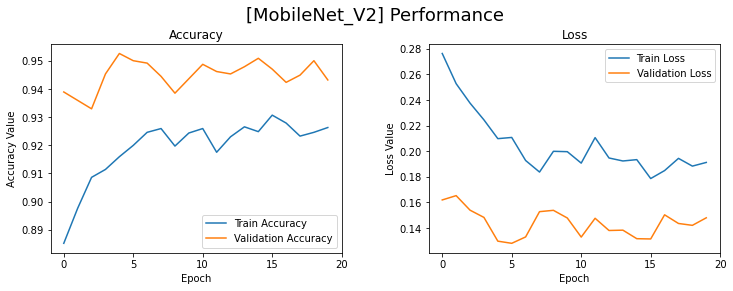
\includegraphics[width=0.7\textwidth]{Images/Modelli/MobileNetV2/MobileNetV2 Pneumonia Performance.png}
                \caption{Performance durante le fasi di \textit{Training} e \textit{Validation} del modello \textit{MobileNetV2} sui Training e Validation datasets di \textit{Chest X-Ray}}
                \label{MobileNetV2 Pneumonia Performance}
            \end{figure}
            
            \begin{figure}[!h]
                \centering
                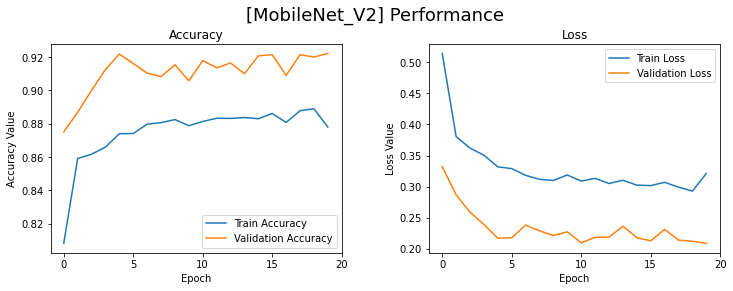
\includegraphics [width=0.7\textwidth]{Images/Modelli/MobileNetV2/MobileNetV2 Brain Performance.png}
                \caption{Performance durante le fasi di \textit{Training} e \textit{Validation} del modello \textit{MobileNetV2} sui Training e Validation datasets di \textit{Brain Tumor MRI}}
                \label{MobileNetV2 Brain Performance}
            \end{figure}
        
        \paragraph{Testing Phase}
        Di seguito si riportano le Confusion Matrices prodotte durante il lavoro di tesi:
            \begin{figure}[!h]
                \centering
                \subfloat[][Confusion Matrix del modello \textit{MobileNetV2} sul Testing dataset di \textit{Chest X-Ray}] {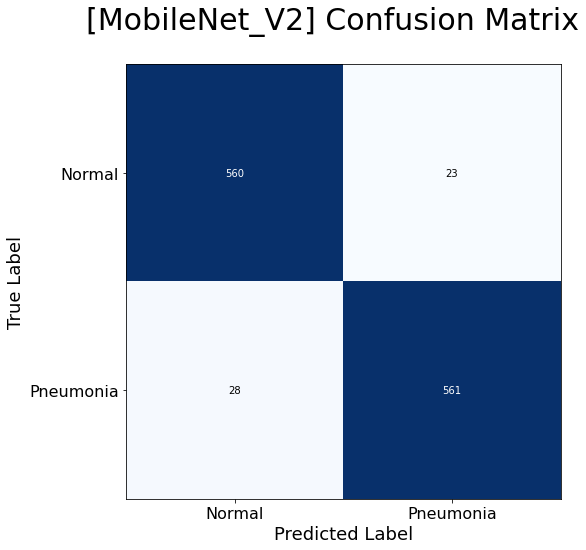
\includegraphics[width=.3\textwidth]{Images/Modelli/MobileNetV2/MobileNetV2 Pneumonia Confusion Matrix.png}} 
                \quad
                \subfloat[][Confusion Matrix del modello \textit{MobileNetV2} sul Testing dataset di \textit{Brain Tumor MRI}] {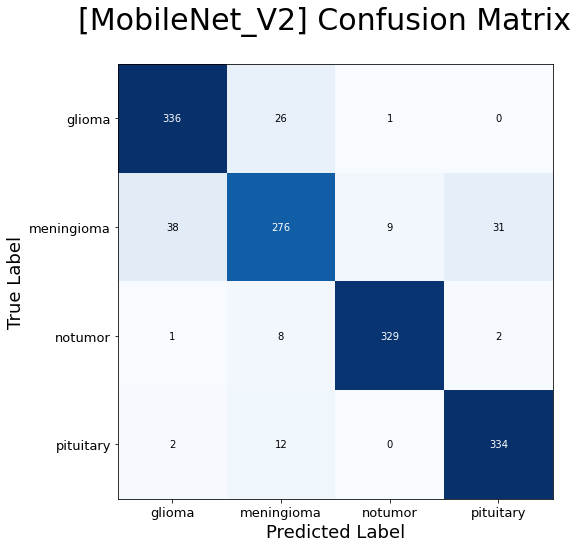
\includegraphics[width=.3\textwidth]{Images/Modelli/MobileNetV2/MobileNetV2 Brain Confusion Matrix.png}}
                \caption{}
                \label{MobileNetV2 Confusion Matrix}
            \end{figure}
        \newpage
        
    \subsection{InceptionV3}
    \label{InceptionV3}
    %[bibl: arXiv:1512.00567]
    Il modello Inception \cite{szegedy2015rethinking}, basandosi sull'uso dei blocchi di costruzione mostrati nella figura \ref{Inception Architecture figures}, mira a cogliere la varietà del dataset evitando un grande consumo di risorse.
    Combinando più filtri di diverse dimensioni allo stesso livello di rete, è possibile catturare informazioni su diverse scale.
        \paragraph{Architettura}
        Di seguito l'architettura del modello InceptionV3:
            \begin{table}[!h]
                \centering
                \begin{tabular}{|c|c|c|}
                    \hline
                    \rule[-3mm]{0mm}{8mm}
                    \textbf{Type} & \textbf{Patch size/stride} & \textbf{Input size}\\
                    & or remarks &\\
                    \hline \hline
                    \rule[-3mm]{0mm}{8mm}
                    conv & 3$\times$3/2 & 299$\times$299$\times$3\\
                    \hline
                    \rule[-3mm]{0mm}{8mm}
                    conv & 3$\times$3/1 & 149$\times$149$\times$32\\
                    \hline
                    \rule[-3mm]{0mm}{8mm}
                    conv padded & 3$\times$3/1 & 147$\times$147$\times$32\\
                    \hline
                    \rule[-3mm]{0mm}{8mm}
                    pool & 3$\times$3/2 & 147$\times$147$\times$64\\
                    \hline
                    \rule[-3mm]{0mm}{8mm}
                    conv & 3$\times$3/1 & 73$\times$73$\times$64\\
                    \hline
                    \rule[-3mm]{0mm}{8mm}
                    conv & 3$\times$3/2 & 71$\times$71$\times$80\\
                    \hline
                    \rule[-3mm]{0mm}{8mm}
                    conv & 3$\times$3/1 & 35$\times$35$\times$192\\
                    \hline
                    \rule[-3mm]{0mm}{8mm}
                    3 $\times$ Inception & As in figure \hyperref[InceptionV3_5]{a} & 35$\times$35$\times$288\\
                    \hline
                    \rule[-3mm]{0mm}{8mm}
                    5 $\times$ Inception & As in figure \hyperref[InceptionV3_6]{b} & 17$\times$17$\times$768\\
                    \hline
                    \rule[-3mm]{0mm}{8mm}
                    2 $\times$ Inception & As in figure \hyperref[InceptionV3_7]{c} & 8$\times$8$\times$1280\\
                    \hline
                    \rule[-3mm]{0mm}{8mm}
                    pool & 8$\times$8 & 8$\times$8$\times$2048\\
                    \hline
                    \rule[-3mm]{0mm}{8mm}
                    linear & logits & 1$\times$1$\times$2048\\
                    \hline
                    \rule[-3mm]{0mm}{8mm}
                    softmax & classifier & 1$\times$1$\times$1000\\
                    \hline
                \end{tabular}
                \label{InceptionV3 Architecture}
            \end{table}
        
            \begin{figure}[!h]
                \centering
                \subfloat[][] {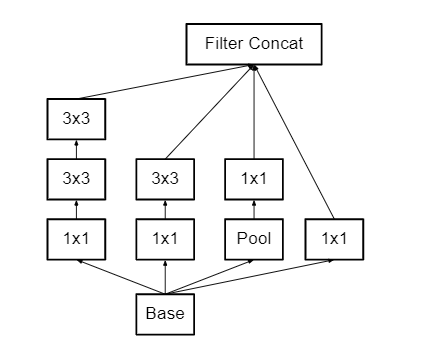
\includegraphics[width=.3\textwidth]{Images/Modelli/InceptionV3/InceptionV3_5.png}} 
                \label{InceptionV3_5}
                \quad
                \subfloat[][] {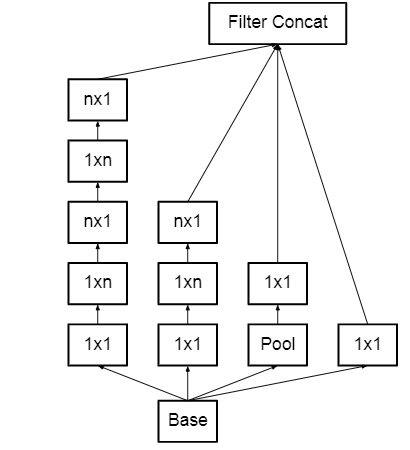
\includegraphics[width=.27\textwidth]{Images/Modelli/InceptionV3/InceptionV3_6.png}} 
                \label{InceptionV3_6}
                \quad
                \subfloat[][] {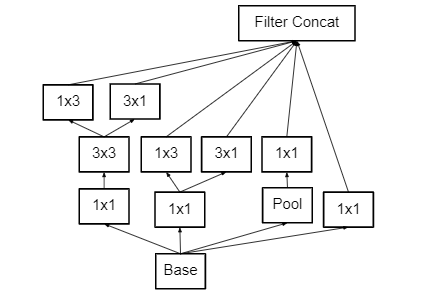
\includegraphics[width=.35\textwidth]{Images/Modelli/InceptionV3/InceptionV3_7.png}}
                \label{InceptionV3_7}
                \caption{}
                \label{Inception Architecture figures}
            \end{figure}
        \newpage
        
        \paragraph{Training and Validation Phase} 
        Di seguito sono riportati i grafici, prodotti durante il lavoro di tesi, raffiguranti le performance del modello, ovvero i valori dell'\textbf{accuracy} e della \textbf{loss} in funzione delle epoche, sia per la fase di \textit{Training} che di \textit{Validation}:
            \begin{figure}[!h]
                \centering
                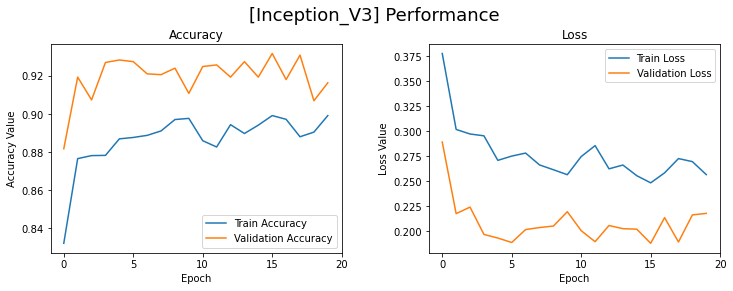
\includegraphics[width=0.7\textwidth]{Images/Modelli/InceptionV3/InceptionV3 Pneumonia Performance.png}
                \caption{Performance durante le fasi di \textit{Training} e \textit{Validation} del modello \textit{InceptionV3} sui Training e Validation datasets di \textit{Chest X-Ray}}
                \label{InceptionV3 Pneumonia Performance}
            \end{figure}
            
            \begin{figure}[!h]
                \centering
                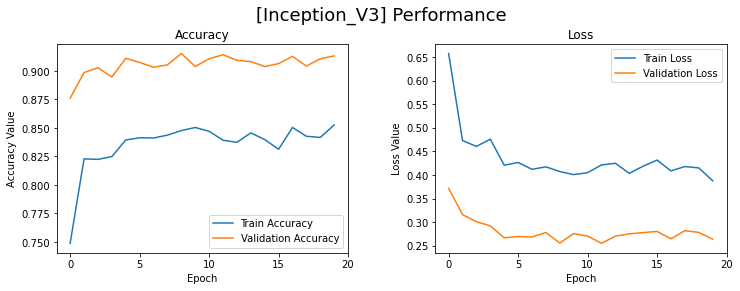
\includegraphics [width=0.7\textwidth]{Images/Modelli/InceptionV3/InceptionV3 Brain Performance.png}
                \caption{Performance durante le fasi di \textit{Training} e \textit{Validation} del modello \textit{InceptionV3} sui Training e Validation datasets di \textit{Brain Tumor MRI}}
                \label{InceptionV3 Brain Performance}
            \end{figure}
        
        \paragraph{Testing Phase}
        Di seguito si riportano le Confusion Matrices prodotte durante il lavoro di tesi:
            \begin{figure}[!h]
                \centering
                \subfloat[][Confusion Matrix del modello \textit{InceptionV3} sul Testing dataset di \textit{Chest X-Ray}] {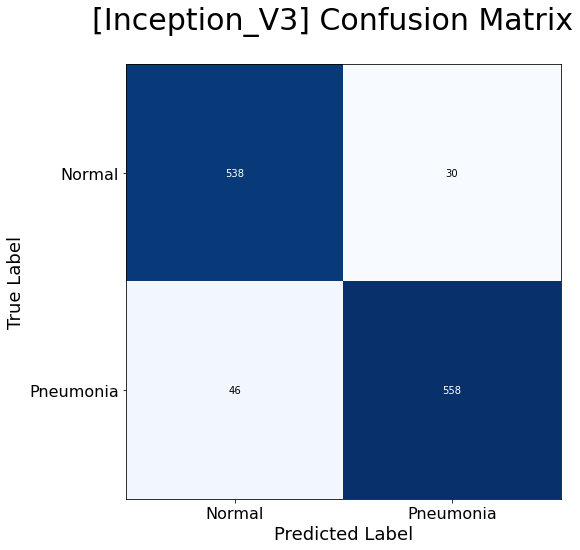
\includegraphics[width=.3\textwidth]{Images/Modelli/InceptionV3/InceptionV3 Pneumonia Confusion Matrix.png}} 
                \quad
                \subfloat[][Confusion Matrix del modello \textit{InceptionV3} sul Testing dataset di \textit{Brain Tumor MRI}] {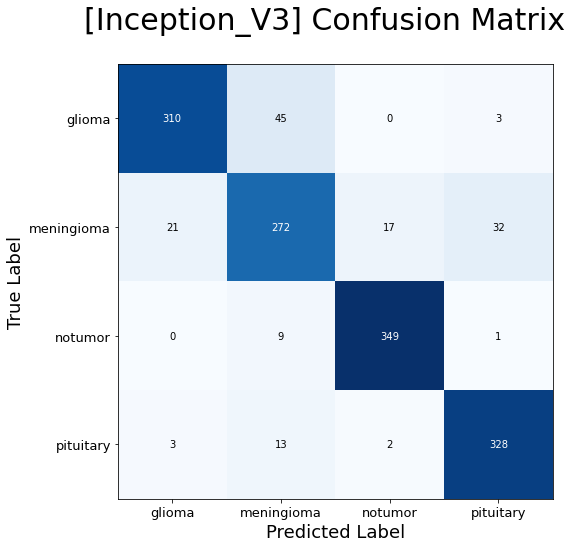
\includegraphics[width=.3\textwidth]{Images/Modelli/InceptionV3/InceptionV3 Brain Confusion Matrix.png}}
                \caption{}
                \label{InceptionV3 Confusion Matrix}
            \end{figure}
    \newpage 
    
\section{Attacchi}
Per eseguire gli attacchi è stata utilizzata la seguente libreria open-source: \\TorchAttacks %[bibl: https://github.com/Harry24k/adversarial-attacks-pytorch]
\cite{kim2020torchattacks}.\\

Si riportano i parametri scelti per i diversi tipi di attacco precedentemente descritti nella sezione \ref{Tecniche di Adversarial Attacks}:
    \begin{table}[!h]
        \centering
        \begin{tabular}{|c|c|}
            \hline
            \rule[-3mm]{0mm}{8mm}
            \textbf{Attack} &\textbf{Parameters used in code} \\ \hline \hline
            \rule[-3mm]{0mm}{8mm}
            FGSM     & $\epsilon=4/255$ \\
            \hline
            \rule[-3mm]{0mm}{8mm}
            BIM      & $\epsilon=4/255,\, \alpha=2/255,\, \text{steps}=100$\\
            \hline
            \rule[-3mm]{0mm}{8mm}
            PGD      & $\epsilon=4/255,\, \alpha=2/255,\, \text{steps}=100$\\
            \hline
            \rule[-3mm]{0mm}{8mm}
            DeepFool & $\text{steps}=50,\, \text{overshoot}=0.02$\\
            \hline
        \end{tabular}
        \caption{}
        \label{Attacks with Parameters}
    \end{table}
    
    La scelta dei parametri è dovuta al grado di percezione del rumore da parte dell'occhio umano. 
    Sono stati scelti i parametri massimi che avrebbero reso la perturbazione impercettibile all'occhio umano.
    Aumentare, anche di poco, i valori dei parametri renderebbe la perturbazione visibile e l'attacco totalmente inefficace perché facilmente rilevabile. 
    
    \newpage
    \subsection{Risultati}
    Di seguito si risportano i risultati degli esperimenti effettuati sugli attacchi durante il lavoro di tesi.
    Si mostra la variazione dell'accuracy dei modelli sulle immagini pulite (No Attacco) e perturbate di entrambi i datasets:
        \begin{table}[!h]
            \centering
            \begin{tabular}{|c||c||c|c|c|c|}
                \hline
                \multicolumn{6}{|c|}{\textbf{Chest X-Ray Dataset}} \rule[-3mm]{0mm}{8mm}\\
                \hline \hline
                \rule[-3mm]{0mm}{8mm}
                \textbf{Modello} & \textbf{No Attacco} & \textbf{FGSM} & \textbf{BIM} & \textbf{PGD} & \textbf{DeepFool} \\
                \hline \hline
                \rule[-3mm]{0mm}{8mm}
                DenseNet121 & 0.9845 & 0.5076  & 0.0000  & 0.0000 & 0.4502\\
                    &  & (-48.44\%) & (-100.0\%) & (-100.0\%) & (-54.27\%)\\
                \hline
                \rule[-3mm]{0mm}{8mm}
                ResNet152   & 0.9811 & 0.4899 & 0.0008 & 0.0017  & 0.4247\\
                    &  & (-50.07\%) & (-99.92\%) & (-99.83\%) & (-56.71\%)\\
                \hline
                \rule[-3mm]{0mm}{8mm}
                VGG19       & 0.9482 & 0.3792  & 0.0000 & 0.0017 & 0.2458\\
                    &  & (-60.01\%) & (-100.0\%) & (-99.82\%) & (-74.08\%)\\
                \hline
                \rule[-3mm]{0mm}{8mm}
                MobileNetV2 & 0.9744 & 0.4780 & 0.0000 & 0.0000 & 0.2534\\
                    &  & (-50.94\%) & (-100.0\%) & (-100.0\%) & (-73.99\%)\\
                \hline
                \rule[-3mm]{0mm}{8mm}
                InceptionV3 & 0.9668 & 0.4899 & 0.0059 & 0.0000 & 0.3446\\
                    &  & (-49.33\%) & (-99.39\%) & (-100.0\%) & (-64.36\%)\\
                \hline
            \end{tabular}
            \caption{Risultati degli attacchi applicati al Testing dataset di \textit{Chest X-Ray}. Ogni cella riporta l'accuracy del modello (riga) sulle immagini perturbate dall'attacco (colonna) e il relativo drop in percentuale rispetto all'accuracy originale.}
            \label{Attacks Results Chest X-Ray}
        \end{table}
        
        \begin{table}[!h]
            \centering
            \begin{tabular}{|c||c||c|c|c|c|}
                \hline
                \multicolumn{6}{|c|}{\textbf{Brain Tumor MRI Dataset}} \rule[-3mm]{0mm}{8mm}\\
                \hline \hline
                \rule[-3mm]{0mm}{8mm}
                \textbf{Modello} & \textbf{No Attacco} & \textbf{FGSM} & \textbf{BIM} & \textbf{PGD} & \textbf{DeepFool} \\
                \hline \hline
                \rule[-3mm]{0mm}{8mm}
                DenseNet121 & 0.9554 & 0.3137 & 0.0007 & 0.0000 & 0.3334 \\
                 & & (-67.17\%) & (-99.93\%) & (-100.0\%) & (-65.10\%)\\
                \hline
                \rule[-3mm]{0mm}{8mm}
                ResNet152   & 0.9332 & 0.4273 & 0.0014 & 0.0000 & 0.4374 \\
                 & & (-54.21\%) & (-99.85\%) & (-100.0\%) & (-53.13\%)\\
                \hline
                \rule[-3mm]{0mm}{8mm}
                VGG19       & 0.9197 & 0.3650 & 0.0156 & 0.0044 & 0.3593 \\
                 & & (-60.31\%) & (-98.30\%) & (-99.52\%) & (-60.93\%)\\
                \hline
                \rule[-3mm]{0mm}{8mm}
                MobileNetV2 & 0.9277 & 0.2789 & 0.0007 & 0.0000 & 0.1564 \\
                 & & (-69.94\%) & (-99.92\%) & (-100.0\%) & (-83.14\%)\\
                \hline
                \rule[-3mm]{0mm}{8mm}
                InceptionV3 & 0.9160 & 0.4598 & 0.0000 & 0.0000 & 0.3659 \\
                 & & (-49.80\%) & (-100.0\%) & (-100.0\%) & (-60.05\%)\\
                \hline
            \end{tabular}
            \caption{Risultati degli attacchi applicati al Testing dataset di \textit{Brain Tumor MRI}. Ogni cella riporta l'accuracy del modello (riga) sulle immagini perturbate dall'attacco (colonna) e il relativo drop in percentuale rispetto all'accuracy originale.}
            \label{Attacks Results Brain Tumor MRI}
        \end{table}
    
    \newpage
    Tutti i 5 modelli considerati sono risultati altamente vulnerabili agli adversarial attacks scelti, con conseguenti diminuzioni significative nell'accuracy dei modelli per entrambi i datasets. 
    
    Gli attacchi più efficaci sono stati BIM e PGD, i quali hanno comportato un calo dell'accuracy, per tutti i modelli e i datasets, superiore al $98\%$.
    Da notare che, a parità di valori assegnati ai parametri ($\epsilon=4/255,\, \alpha=2/255,\, \text{steps}=100$), l'attacco PGD risulta, anche se di poco, più forte di BIM.
    
    Il modello più debole per la classificazione binaria (due sole classi) è VGG19, mentre per la classificazione multiclass (con 3 o più classi) è MobileNetV2. I due modelli, se attaccati, non riescono a raggiungere rispettivamente il 40\% e il 30\% di accuracy. 
    Inoltre, gli attacchi hanno un tasso di successo maggiore sul testing dataset di \textit{Brain Tumor MRI}. Si osserva che, a parità di perturbazioni, l'accuratezza dei vari modelli sugli adversarial examples diminuisce all'aumentare del numero di classi. Ciò significa che i datasets multiclass sono più vulnerabili rispetto a quelli binari.
    
    \newpage
    Si riportano di seguito alcuni esempi di classificazione errata:
        \begin{figure}[!h]
            \centering
            \subfloat[][8 esempi con rispettive classi reali e predizioni del modello \textit{DenseNet121} su immagini perturbate con l'attacco PGD del Testing dataset di \textit{Brain Tumor MRI}] {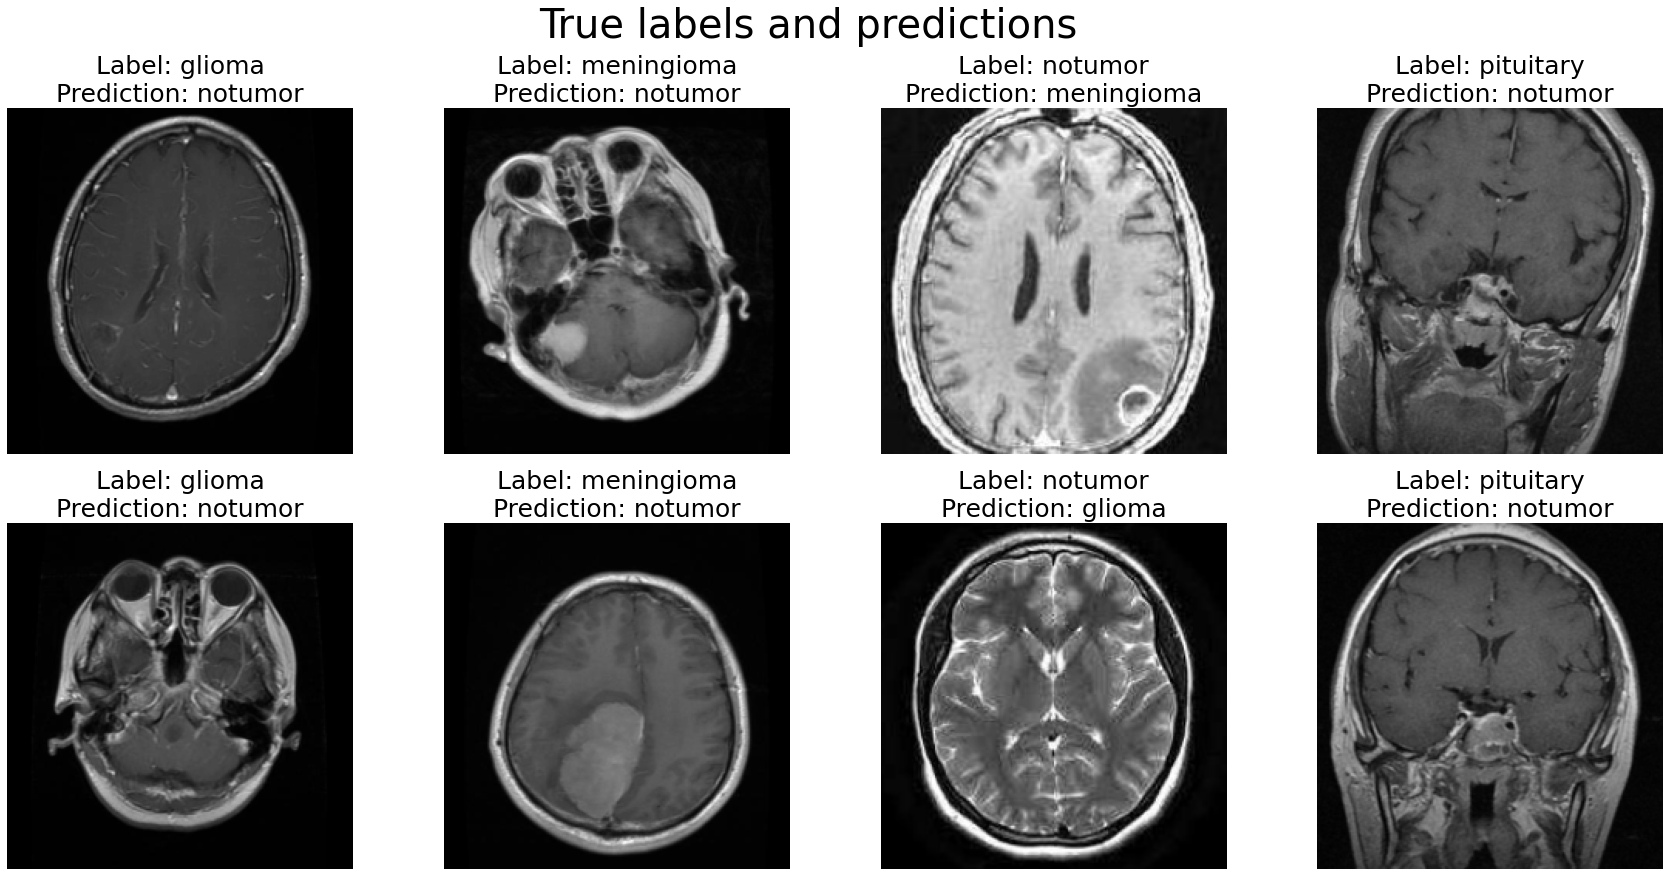
\includegraphics[width=\textwidth]{Images/Esempi attacchi/Brain MRI/Densenet121 Brain PGD 8 True&Predictions.png}}
            \quad
            \subfloat[][10 esempi con rispettive classi reali e predizioni del modello \textit{DenseNet121} su immagini perturbate con l'attacco PGD del Testing dataset di \textit{Chest X-Ray}] {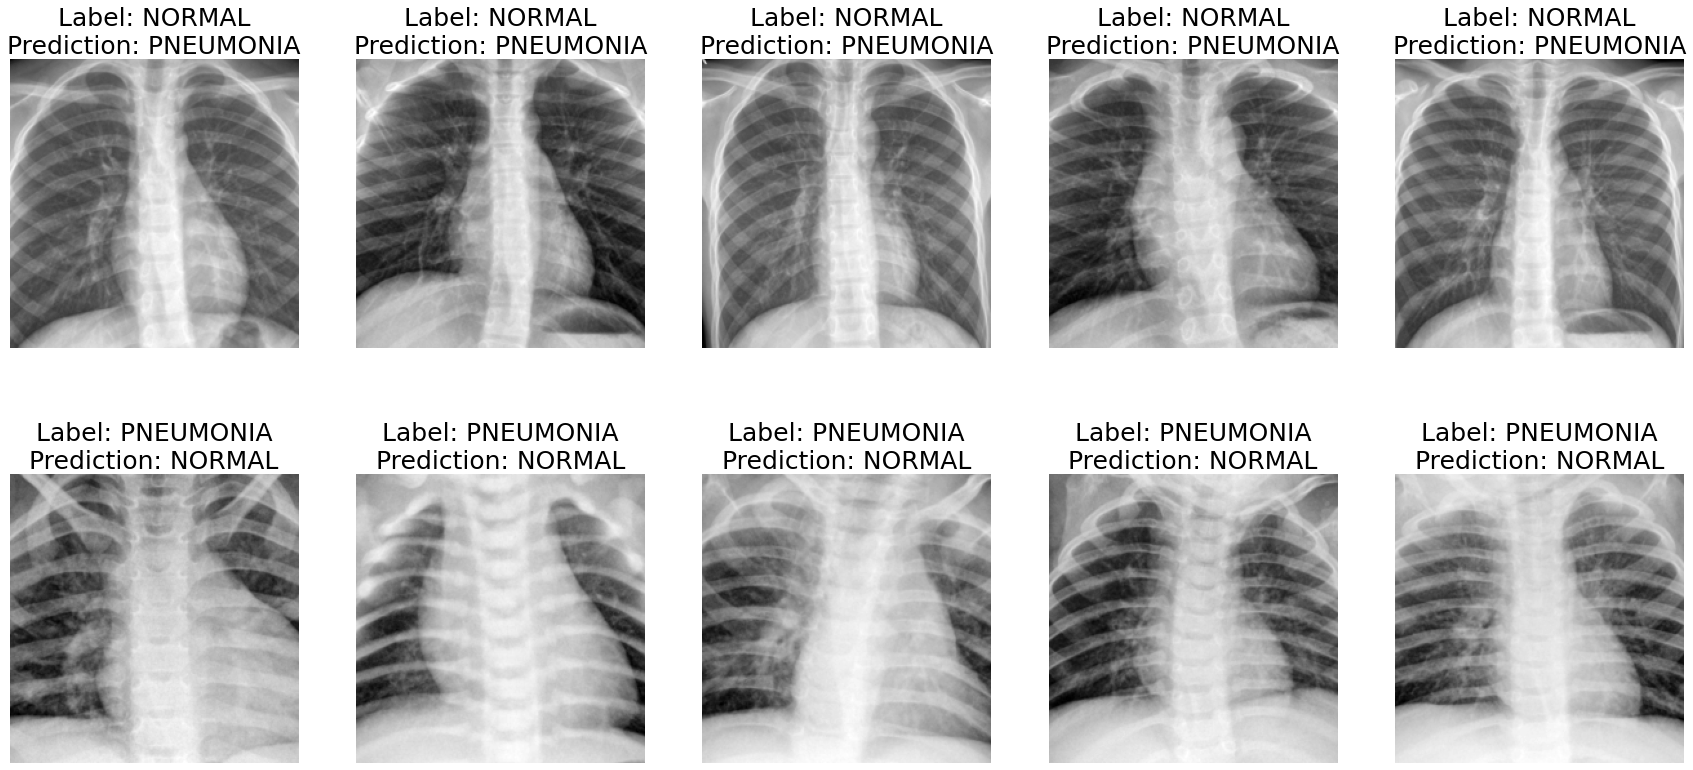
\includegraphics[width=\textwidth]{Images/Esempi attacchi/Pneumonia/DenseNet121 Pneumonia PGD 10 True&Predictions.png}} 
            \caption{}
            \label{DenseNet121 wrong predictions}
        \end{figure}
    
    \newpage
    Di seguito alcune immagini che raffigurano le perturbazioni e gli adversarial examples prodotti dagli attacchi sul Testing dataset di \textit{Chest X-Ray}:
        
        \begin{figure}[!h]
            \centering
            
            \quad
            \subfloat[][Originale] {\includegraphics[width=.25\textwidth]{Images/Esempi attacchi/Pneumonia/FGSM_Clean.png}} 
            \quad
            \subfloat[][Perturbata\\ (FGSM)] {\includegraphics[width=.25\textwidth]{Images/Esempi attacchi/Pneumonia/FGSM_Perturbated.png}}
            \quad
            \subfloat[][Perturbazione\\ (FGSM)] {\includegraphics[width=.25\textwidth]{Images/Esempi attacchi/Pneumonia/FGSM_Noise.png}}
            
            \quad
            \subfloat[][Originale] {\includegraphics[width=.25\textwidth]{Images/Esempi attacchi/Pneumonia/BIM_Clean.png}} 
            \quad
            \subfloat[][Perturbata\\ (BIM)] {\includegraphics[width=.25\textwidth]{Images/Esempi attacchi/Pneumonia/BIM_Perturbated.png}}
            \quad
            \subfloat[][Perturbazione\\ (BIM)] {\includegraphics[width=.25\textwidth]{Images/Esempi attacchi/Pneumonia/BIM_Noise.png}}
            
            \quad
            \subfloat[][Originala] {\includegraphics[width=.25\textwidth]{Images/Esempi attacchi/Pneumonia/PGD_Clean.png}} 
            \quad
            \subfloat[][Perturbata\\ (PGD)] {\includegraphics[width=.25\textwidth]{Images/Esempi attacchi/Pneumonia/PGD_Perturbated.png}}
            \quad
            \subfloat[][Perturbazione\\ (PGD)] {\includegraphics[width=.25\textwidth]{Images/Esempi attacchi/Pneumonia/PGD_Noise.png}}
            
            \quad
            \subfloat[][Originale] {\includegraphics[width=.25\textwidth]{Images/Esempi attacchi/Pneumonia/DeepFool_Clean.png}} 
            \quad
            \subfloat[][Perturbata\\ (DeepFool)] {\includegraphics[width=.25\textwidth]{Images/Esempi attacchi/Pneumonia/DeepFool_Perturbated.png}}
            \quad
            \subfloat[][Perturbazione\\ (DeepFool)] {\includegraphics[width=.25\textwidth]{Images/Esempi attacchi/Pneumonia/DeepFool_Noise.png}}
            
            \caption{Esempi di perturbazioni create per ingannare il modello \textit{DenseNet121} su immagini del Testing dataset di \textit{Chest X-Ray}. Ogni riga rappresenta un attacco diverso e si compone di 3 immagini: l'immagine originale e pulita, l'adversarial example corrispondente, la perturbazione aggiunta alla prima immagine per produrre la seconda.}
            \label{Attacks Examples Chest X-Ray}
        \end{figure}
    
    \newpage    
    Di seguito alcune immagini che raffigurano le perturbazioni e gli adversarial examples prodotti dagli attacchi sul Testing dataset di \textit{Brain Tumor MRI}:
        \begin{figure}[!h]
            \centering
            
            \quad
            \subfloat[][Originale] {\includegraphics[width=.25\textwidth]{Images/Esempi attacchi/Brain MRI/FGSM_Clean.png}} 
            \quad
            \subfloat[][Perturbata\\ (FGSM)] {\includegraphics[width=.25\textwidth]{Images/Esempi attacchi/Brain MRI/FGSM_Perturbated.png}}
            \quad
            \subfloat[][Perturbazione\\ (FGSM)] {\includegraphics[width=.25\textwidth]{Images/Esempi attacchi/Brain MRI/FGSM_Noise.png}}
            
            \quad
            \subfloat[][Originale] {\includegraphics[width=.25\textwidth]{Images/Esempi attacchi/Brain MRI/BIM_Clean.png}} 
            \quad
            \subfloat[][Perturbata\\ (BIM)] {\includegraphics[width=.25\textwidth]{Images/Esempi attacchi/Brain MRI/BIM_Perturbated.png}}
            \quad
            \subfloat[][Perturbazione\\ (BIM)] {\includegraphics[width=.25\textwidth]{Images/Esempi attacchi/Brain MRI/BIM_Noise.png}}
            
            \quad
            \subfloat[][Originale] {\includegraphics[width=.25\textwidth]{Images/Esempi attacchi/Brain MRI/PGD_Clean.png}} 
            \quad
            \subfloat[][Perturbata\\ (PGD)] {\includegraphics[width=.25\textwidth]{Images/Esempi attacchi/Brain MRI/PGD_Perturbated.png}}
            \quad
            \subfloat[][Perturbazione\\ (PGD)] {\includegraphics[width=.25\textwidth]{Images/Esempi attacchi/Brain MRI/PGD_Noise.png}}
            
            \quad
            \subfloat[][Originale] {\includegraphics[width=.25\textwidth]{Images/Esempi attacchi/Brain MRI/DeepFool_Clean.png}} 
            \quad
            \subfloat[][Perturbata\\ (DeepFool)] {\includegraphics[width=.25\textwidth]{Images/Esempi attacchi/Brain MRI/DeepFool_Perturbated.png}}
            \quad
            \subfloat[][Perturbazione\\ (DeepFool)] {\includegraphics[width=.25\textwidth]{Images/Esempi attacchi/Brain MRI/DeepFool_Noise.png}}
            
            \caption{Esempi di perturbazioni create per ingannare il modello \textit{DenseNet121} su immagini del Testing dataset di \textit{Brain Tumor MRI}. Ogni riga rappresenta un attacco diverso e si compone di 3 immagini: l'immagine originale e pulita, l'adversarial example corrispondente, la perturbazione aggiunta alla prima immagine per produrre la seconda.}
            \label{Attacks Examples Brain Tumor MRI}
        \end{figure}

\chapter{Mitigation di Adversarial Attacks: esperimenti}
\label{chap:5}
Durante il lavoro di tesi sono state testate due delle tecniche di mitigation di adversarial attacks illustrate nella sezione \ref{C3: Mitigation}:
    \begin{itemize}
        \item Adversarial Training (\ref{BF Adversarial Training}): testato su un solo modello (DenseNet121), un solo attacco (FGSM) ed entrambi i datasets. 
        \item Pix2Pix GAN (\ref{Pix2Pix GAN}): testato su tutti i modelli, tutti gli attacchi ed entrambi i datasets.
    \end{itemize}
    
    Le scelte adottate sono dovute alla valutazione di tempi e costi computazionali richiesti per l'applicazione dei metodi. L'Adversarial Training, a differenza della GAN, richiede un raddoppio della dimensione del Training dataset e, di conseguenza, un significativo aumento di tempo e risorse investite nella fase di training del modello.
    
    Inoltre, durante l'esecuzione degli esperimenti è emerso che l'utilizzo dell'Adversarial Training comportava un drop dell'accuracy del modello sulle immagini pulite del Testing dataset.

\newpage
\section{Adversarial Training}
    Di seguito si riportano i risultati degli esperimenti effettuati.
    Si confrontano le due tecniche di training prese in esame: Hold-out Training (\ref{Hold-Out method}) e Adversarial Training. 
    Si mostra la variazione dell'accuracy del modello DenseNet121 sulle immagini pulite (No Attacco) e perturbate di entrambi i datasets:
    \begin{table}[!h]
        \centering
        \begin{tabular}{|c||c|c|}
            \hline
            \multicolumn{3}{|c|}{\textbf{Chest X-Ray Dataset}} \rule[-3mm]{0mm}{8mm}\\
            \hline
            \rule[-3mm]{0mm}{8mm}
            & \textbf{No Attacco} & \textbf{FGSM}\\
            \hline \hline
            \rule[-3mm]{0mm}{8mm}
            \textbf{Hold-Out Training}      & 0.9845 & 0.5076 \\
             & & (-48.44\%) \\
            \hline
            \rule[-3mm]{0mm}{8mm}
            \textbf{Adversarial Training}   & 0.9020 & 0.8003 \\
             & &  (-11.27\%)\\
            \hline
        \end{tabular}
        \caption{\textit{Adversarial Training} del modello \textit{DenseNet121} sul dataset \textit{Chest X-Ray}}
        \label{Adversarial Training Chest X-Ray}
    \end{table}
    
    \begin{table}[!h]
        \centering
        \begin{tabular}{|c||c|c|}
            \hline
            \multicolumn{3}{|c|}{\textbf{Brain Tumor MRI Dataset}} \rule[-3mm]{0mm}{8mm}\\
            \hline
            \rule[-3mm]{0mm}{8mm}
            & \textbf{No Attacco} & \textbf{FGSM}\\
            \hline \hline
            \rule[-3mm]{0mm}{8mm}
            \textbf{Hold-Out Training}      & 0.9554 & 0.3137 \\
             & & (-67.17\%) \\
            \hline
            \rule[-3mm]{0mm}{8mm}
            \textbf{Adversarial Training }  & 0.8876 & 0.7697 \\
             & & (-13.28\%) \\
            \hline
        \end{tabular}
        \caption{\textit{Adversarial Training} del modello \textit{DenseNet121} sul dataset \textit{Brain Tumor MRI}}
        \label{Adversarial Training Brain Tumor MRI}
    \end{table}
    
I risultati dimostrano che, sebbene i modelli siano estremamente sensibili agli adversarial attacks, l'adversarial training mostra la premessa per lo sviluppo di una difesa efficace contro gli attacchi. La vulnerabilità delle singole immagini può essere usata per aumentare le prestazioni del modello identificando le immagini più a rischio di errore di classificazione.

Tuttavia, il metodo rimane di difficile applicazione a causa degli elevati tempi e costi computazionali richiesti.

Inoltre, nonostante il modello risulti più robusto durante la fase di testing su immagini perturbate, l'accuracy generale su immagini pulite subisce un calo consistente, di circa il $10\%$.

\newpage
\section{Architettura della Pix2Pix GAN}
L'architettura della GAN utilizzata durante il lavoro di tesi è tratta da %[bibl: https://arxiv.org/pdf/1611.07004.pdf] 
\cite{isola2016image}:
    %\paragraph{Architettura del Generator}
        \begin{table}[!h]
            \centering
            \begin{tabular}{|c|c||c|c|}
                \hline
                \multicolumn{4}{|c|}{\textbf{Generator}} \rule[-3mm]{0mm}{8mm}\\
                \hline \hline
                \multicolumn{2}{|c||}{\textbf{Encoder}} & 
                \multicolumn{2}{|c|}{\textbf{U-Net Decoder}} \rule[-3mm]{0mm}{8mm}\\
                \hline \hline
                \rule[-3mm]{0mm}{8mm}
                \textbf{Layers} & \textbf{Output size} & \textbf{Layers} & \textbf{Output size}\\
                \hline
                \rule[-3mm]{0mm}{8mm}
                C64 & $128 \times 128$      & CD512 & $2 \times 2$ \\
                lReLU(0.2)      &                & BN + ReLU + Dropout(0.5) & \\
                \hline
                \rule[-3mm]{0mm}{8mm}
                C128 & $64 \times 64$       & CD1024 & $4 \times 4$ \\
                BN + lReLU(0.2) &                & BN + ReLU + Dropout(0.5) & \\
                \hline
                \rule[-3mm]{0mm}{8mm}
                C256 & $32 \times 32$       & CD1024 & $8 \times 8$ \\
                BN + lReLU(0.2) &                & BN + ReLU + Dropout(0.5) & \\
                \hline
                \rule[-3mm]{0mm}{8mm}
                C512 & $16 \times 16$       & CD1024 & $16 \times 16$ \\
                BN + lReLU(0.2) &                & BN + ReLU + Dropout(0.5) & \\
                \hline
                \rule[-3mm]{0mm}{8mm}
                C512 & $8 \times 8$         & CD1024 & $32 \times 32$ \\
                BN + lReLU(0.2) &                & BN + ReLU + Dropout(0.5) & \\
                \hline
                \rule[-3mm]{0mm}{8mm}
                C512 & $4 \times 4$         & CD512 & $64 \times 64$ \\
                BN + lReLU(0.2) &                & BN + ReLU + Dropout(0.5) & \\
                \hline
                \rule[-3mm]{0mm}{8mm}
                C512 & $2 \times 2$         & CD256 & $128 \times 128$ \\
                BN + lReLU(0.2) &                & BN + ReLU + Dropout(0.5) & \\
                \hline
                \rule[-3mm]{0mm}{8mm}
                C512 & $1 \times 1$         & CD128 & $256 \times 256$ \\
                lReLU(0.2)      &                & BN + ReLU + Dropout(0.5) & \\
                \hline
            \end{tabular}
            \caption{Architettura del Generator. 
            C$k$: Convolutional layer con $k$ $4 \times 4$ filtri e $stride=2$. BN: BatchNorm. 
            CD$k$: ConvTranspose2d layer con $k$ $4 \times 4$ filtri e $stride=2$. \\
            Activation function del Generator: $Tanh$}
            \label{Generator Architecture}
        \end{table}

\newpage
        \begin{table}[!h]
            \centering
            \begin{tabular}{|c|c|}
                \hline
                \multicolumn{2}{|c|}{\textbf{Discriminator $70 \times 70$}} \rule[-3mm]{0mm}{8mm}\\
                \hline \hline
                \rule[-3mm]{0mm}{8mm}
                \textbf{Layers} & \textbf{Output size} \\
                \hline \hline
                \rule[-3mm]{0mm}{8mm}
                C64                 & $128 \times 128$  \\
                lReLU(0.2) & \\
                \hline
                \rule[-3mm]{0mm}{8mm}
                C128                & $64 \times 64$  \\
                BN + lReLU(0.2) & \\
                \hline
                \rule[-3mm]{0mm}{8mm}
                C256                & $32 \times 32$  \\
                BN + lReLU(0.2) & \\
                \hline
                \rule[-3mm]{0mm}{8mm}
                C512                & $31 \times 31$  \\
                BN + lReLU(0.2) & \\
                \hline
                \rule[-3mm]{0mm}{8mm}
                C1                & $30 \times 30$  \\
                lReLU(0.2) & \\
                \hline
            \end{tabular}
            \caption{Architettura del Discriminator. 
            C$k$: Convolutional layer con $k$ $4 \times 4$ filtri e $stride=2$. BN: BatchNorm. \\
            Activation function del Discriminator: $Sigmoid$}
            \label{Discriminator architecture}
        \end{table}
    
    \subsection{Risultati}
    
        \begin{table}[!h]
                \centering
                \begin{tabular}{|c||c|c|c|c|c|}
                    \hline
                    \multicolumn{6}{|c|}{\textbf{Chest X-Ray Dataset}} \rule[-3mm]{0mm}{8mm}\\
                    \hline \hline
                    \rule[-3mm]{0mm}{8mm}
                    \textbf{Model} & \textbf{No Attacco} & \textbf{FGSM} & \textbf{BIM} & \textbf{PGD} & \textbf{DeepFool} \\
                    \hline \hline
                    \rule[-3mm]{0mm}{8mm}
                    DenseNet121 & 0.9845 & 0.8794 & 0.8167 & 0.7903 & 0.8423\\
                        &  & (-10.68\%) & (-17.04\%) & (-19.73\%) & (-14.44\%)\\
                    \hline
                    \rule[-3mm]{0mm}{8mm}
                    ResNet152   & 0.9811 & 0.8154 & 0.7997 & 0.7776  & 0.7901\\
                        &  & (-16.89\%) & (-18.49\%) & (-20.74\%) & (-19.47\%)\\
                    \hline
                    \rule[-3mm]{0mm}{8mm}
                    VGG19       & 0.9482 & 0.6287 & 0.5893 & 0.5608 & 0.6339\\
                        &  & (-33.70\%) & (-37.85\%) & (-40.86\%) & (-33.15\%)\\
                    \hline
                    \rule[-3mm]{0mm}{8mm}
                    MobileNetV2 & 0.9744 & 0.7963 & 0.7348 & 0.7096 & 0.8055\\
                        &  & (-18.28\%) & (-24.59\%) & (-27.18\%) & (-17.33\%)\\
                    \hline
                    \rule[-3mm]{0mm}{8mm}
                    InceptionV3 & 0.9668 & 0.8094 & 0.7728 & 0.7418 & 0.7904\\
                        &  & (-16.28\%) & (-20.07\%) & (-23.27\%) & (-18.25\%)\\
                    \hline
                \end{tabular}
                \caption{Risultati dell'utilizzo della GAN per mitigare gli attacchi applicati al dataset \textit{Chest X-Ray}.
                Ogni cella riporta l'accuracy del modello (riga) sulle immagini perturbate dall'attacco (colonna) e il relativo drop in percentuale rispetto all'accuracy originale.}
                \label{Mitigation Results Chest X-Ray}
            \end{table}
            
            \newpage
            \begin{table}[!h]
                \centering
                \begin{tabular}{|c||c|c|c|c|c|}
                    \hline
                    \multicolumn{6}{|c|}{\textbf{Brain Tumor MRI Dataset}} \rule[-3mm]{0mm}{8mm}\\
                    \hline \hline
                    \rule[-3mm]{0mm}{8mm}
                    \textbf{Model} & \textbf{No Attacco} & \textbf{FGSM} & \textbf{BIM} & \textbf{PGD} & \textbf{DeepFool} \\
                    \hline \hline
                    \rule[-3mm]{0mm}{8mm}
                    DenseNet121 & 0.9554 & 0.8689 & 0.8298 & 0.8046 & 0.8577 \\
                     & & (-9.05\%) & (-13.15\%) & (-15.78\%) & (-10.23\%)\\
                    \hline
                    \rule[-3mm]{0mm}{8mm}
                    ResNet152   & 0.9332 & 0.8220 & 0.7845 & 0.7565 & 0.8126 \\
                     & & (-11.92\%) & (-15.93\%) & (-18.93\%) & (-12.92\%)\\
                    \hline
                    \rule[-3mm]{0mm}{8mm}
                    VGG19       & 0.9197 & 0.6390 & 0.6074 & 0.5545 & 0.6134 \\
                     & & (-30.52\%) & (-33.96\%) & (-39.71\%) & (-33.30\%)\\
                    \hline
                    \rule[-3mm]{0mm}{8mm}
                    MobileNetV2 & 0.9277 & 0.8035 & 0.7532 & 0.7299 & 0.7943 \\
                     & & (-13.39\%) & (-18.81\%) & (-21.32\%) & (-14.38\%)\\
                    \hline
                    \rule[-3mm]{0mm}{8mm}
                    InceptionV3 & 0.9160 & 0.7923 & 0.7789 & 0.7302 & 0.7907 \\
                     & & (-13.50\%) & (-14.97\%) & (-20.28\%) & (-13.68\%)\\
                    \hline
                \end{tabular}
                \caption{Risultati dell'utilizzo della GAN per mitigare gli attacchi applicati al dataset \textit{Brain Tumor MRI}.
                Ogni cella riporta l'accuracy del modello (riga) sulle immagini perturbate dall'attacco (colonna) e il relativo drop in percentuale rispetto all'accuracy originale.}
                \label{Mitigation Results Brain Tumor MRI}
            \end{table}
            
            L'impiego della GAN ha sicuramente portato dei miglioramenti nell'accuracy dei modelli, risultando un metodo di difesa valido.
            
            L'efficacia di attacchi in grado di azzerare l'accuracy dei modelli, BIM e PGD, è ridotta in modo significativo. In questi casi l'accuracy è stata riportata a valori solidi compresi tra 70-80\%.
            
            Oltre ad essere il modello più vulnerabile, VGG19 è anche il più difficile da difendere, indipendentemente dal tipo di attacco utilizzato. Al contempo, il modello che performa meglio, se difeso, è DenseNet121.
            
            Si noti che tutti i modelli hanno raggiunto livelli di performance superiori durante la classificazione effettuata sulle immagini del dataset con 4 classi. Si deduce che i datasets multiclass, anche se più vulnerabili, siano più facili da difendere rispetto a quelli binari.   
            
            In generale, l'utilizzo della GAN riesce a mitigare gli adversarial attacks in modo più efficace rispetto all'Adversarial Training. Inoltre, non venendo apportate modifiche alla fase di training del modello, durante la fase di testing, l'accuracy dei modelli sulle immagini pulite dei datasets rimane invariata. 
            
            \newpage
            Di seguito si riporta l'aumento dell’accuracy dei modelli in seguito all’utilizzo della GAN per mitigare gli attacchi:
            
            \begin{table}[!h]
                \centering
                \begin{tabular}{|c||c|c|c|c|c|}
                    \hline
                    \multicolumn{6}{|c|}{\textbf{Chest X-Ray Dataset}} \rule[-3mm]{0mm}{8mm}\\
                    \hline \hline
                    \rule[-3mm]{0mm}{8mm}
                    \textbf{Model} & \textbf{No Attacco} & \textbf{FGSM} & \textbf{BIM} & \textbf{PGD} & \textbf{DeepFool} \\
                    \hline \hline
                    \rule[-3mm]{0mm}{8mm}
                    DenseNet121 & 0.9845 & 0.5076  & 0.0000  & 0.0000 & 0.4502\\
                                       & & 0.8794 & 0.8167 & 0.7903 & 0.8423\\
                     \rule[-3mm]{0mm}{8mm}
                     & & (+0.3718) & (+0.8167) & (+0.7903) & (+0.3903)\\
                    \hline
                    \rule[-3mm]{0mm}{8mm}
                    ResNet152 & 0.9811 & 0.4899 & 0.0008 & 0.0017  & 0.4247\\
                                     & & 0.8154 & 0.7997 & 0.7776  & 0.7901\\
                     \rule[-3mm]{0mm}{8mm}
                     & & (+0.3255) & (+0.7989) & (+0.7759) & (+0.3654)\\
                    \hline
                    \rule[-3mm]{0mm}{8mm}
                    VGG19 & 0.9482 & 0.3792 & 0.0000 & 0.0017 & 0.2458\\
                                 & & 0.6287 & 0.5893 & 0.5608 & 0.6339\\
                     \rule[-3mm]{0mm}{8mm}
                     & & (+0.2495) & (+0.5893) & (+0.5591) & (+0.3881)\\
                    \hline
                    \rule[-3mm]{0mm}{8mm}
                    MobileNetV2 & 0.9744 & 0.4780 & 0.0000 & 0.0000 & 0.2534\\
                                       & & 0.7963 & 0.7348 & 0.7096 & 0.8055\\
                     \rule[-3mm]{0mm}{8mm}
                     & & (+0.3183) & (+0.7348) & (+0.7096) & (+0.5521)\\
                    \hline
                    \rule[-3mm]{0mm}{8mm}
                    InceptionV3 & 0.9668 & 0.4899 & 0.0059 & 0.0000 & 0.3446\\
                                       & & 0.8094 & 0.7728 & 0.7418 & 0.7904\\ 
                     \rule[-3mm]{0mm}{8mm}
                     & & (+0.3195) & (+0.7669) & (+0.7418) & (+0.4458)\\
                    \hline
                \end{tabular}
                \caption{Aumento dell'accuracy dei modelli in seguito all'utilizzo della GAN per mitigare gli attacchi applicati al dataset \textit{Chest X-Ray}.
                Ogni cella riporta l'accuracy del modello (riga) sulle immagini perturbate dall'attacco (colonna) senza e con l'impiego della GAN, e l'aumento dell'accuracy.}
                \label{Rise accuracy Chest X-Ray}
            \end{table}
            
            \newpage
            \begin{table}[!h]
                \centering
                \begin{tabular}{|c||c|c|c|c|c|}
                    \hline
                    \multicolumn{6}{|c|}{\textbf{Brain Tumor MRI Dataset}} \rule[-3mm]{0mm}{8mm}\\
                    \hline \hline
                    \rule[-3mm]{0mm}{8mm}
                    \textbf{Model} & \textbf{No Attacco} & \textbf{FGSM} & \textbf{BIM} & \textbf{PGD} & \textbf{DeepFool} \\
                    \hline \hline
                    \rule[-3mm]{0mm}{8mm}
                    DenseNet121 & 0.9554 & 0.3137 & 0.0007 & 0.0000 & 0.3334 \\
                                       & & 0.8689 & 0.8298 & 0.8046 & 0.8577 \\
                    \rule[-3mm]{0mm}{8mm}
                     & & (+0.5552) & (+0.8291) & (+0.8046) & (+0.5243)\\
                    \hline
                    \rule[-3mm]{0mm}{8mm}
                    ResNet152   & 0.9332 & 0.4273 & 0.0014 & 0.0000 & 0.4374 \\ 
                                       & & 0.8220 & 0.7845 & 0.7565 & 0.8126 \\
                    \rule[-3mm]{0mm}{8mm}
                     & & (+0.3947) & (+0.7831) & (+0.7565) & (+0.3752)\\
                    \hline
                    \rule[-3mm]{0mm}{8mm}
                    VGG19       & 0.9197 & 0.3650 & 0.0156 & 0.0044 & 0.3593 \\
                                       & & 0.6390 & 0.6074 & 0.5545 & 0.6134 \\
                    \rule[-3mm]{0mm}{8mm} 
                     & & (+0.2740) & (+0.5918) & (+0.5501) & (+0.2541)\\
                    \hline
                    \rule[-3mm]{0mm}{8mm}
                    MobileNetV2 & 0.9277 & 0.2789 & 0.0007 & 0.0000 & 0.1564 \\
                                       & & 0.8035 & 0.7532 & 0.7299 & 0.7943 \\ 
                    \rule[-3mm]{0mm}{8mm}
                     & & (+0.5246) & (+0.7525) & (+0.7299) & (+0.6379)\\
                    \hline
                    \rule[-3mm]{0mm}{8mm}
                    InceptionV3 & 0.9160 & 0.4598 & 0.0000 & 0.0000 & 0.3659 \\
                                       & & 0.7923 & 0.7789 & 0.7302 & 0.7907 \\
                    \rule[-3mm]{0mm}{8mm}
                     & & (+0.3325) & (+0.7789) & (+0.7302) & (+0.4249)\\
                    \hline
                \end{tabular}
                \caption{Aumento dell'accuracy dei modelli in seguito all'utilizzo della GAN per mitigare gli attacchi applicati al dataset \textit{Brain Tumor MRI}.
                Ogni cella riporta l'accuracy del modello (riga) sulle immagini perturbate dall'attacco (colonna) senza e con l'impiego della GAN, e l'aumento dell'accuracy.}
                \label{Rise accuracy Brain Tumor MRI}
            \end{table}

\chapter{Conclusioni}

Il Deep Learning (DL) ha notevolmente migliorato l'analisi delle immagini mediche ed è diventato uno strumento indispensabile per medici e operatori sanitari. Tuttavia, gli adversarial attacks ostacolano il corretto funzionamento dei modelli di DL, mettendo in serio pericolo le vite dei pazienti.\\

Nell'elaborato presentato, è stato analizzato il problema degli adversarial attacks sul riconoscimento delle immagini mediche. 

Sono stati condotti una serie di esperimenti con 5 modelli CNN, 4 tipi di attacchi e 2 tecniche di difesa su 2 datasets di immagini mediche, rispettivamente di 2 e 4 classi.

Nessuno dei modelli proposti si è rivelato abbastanza robusto e sicuro da resistere agli adversarial attacks scelti.
Gli attacchi applicati si sono dimostrati, nonostante la loro semplicità, estremamente efficaci. In alcuni casi hanno persino comportato un calo dell'accuracy dei modelli del 100\%.
 
Anche se i metodi di difesa adottati per contrastare gli adversarial attacks hanno ottenuto buoni risultati, che possono ridurre consistentemente il tasso di successo dell'attacco, sono generalmente rivolti ad un tipo specifico di attacco. 
Nel complesso non esiste un metodo di difesa in grado di proteggere un modello da qualsiasi tipo di attacco.
Inoltre, anche se difeso, il modello attaccato non riesce a ripristinare l'accuracy originale che raggiungerebbe su un dataset di immagini pulite in input.\\

Pertanto, la chiave per garantire la sicurezza dei modelli di DL è quella di continuare le ricerche in maniera approfondita sui metodi di adversarial attacks e proporre strategie di difesa più efficienti.

\backmatter
\phantomsection

\bibliographystyle{sapthesis}
\bibliography{Bibliografia}

\end{document}